% \begin{name}
% 	{GV biên soạn: Nguyễn Tuấn\\ GV phản biện: Nguyễn Văn B}
% 	{TOÁN 10-KNTT-CS}
% \end{name}
%----------------NỘI DUNG BIÊN SOẠN
\newpage
\setcounter{section}{1}
\setcounter{dang}{0}
\def\tenchude{TẬP HỢP VÀ CÁC PHÉP TOÁN TRÊN TẬP HỢP}
\section{TẬP HỢP VÀ CÁC PHÉP TOÁN TRÊN TẬP HỢP}


%-------------------------------------------
\subsection{KIẾN THỨC TRỌNG TÂM}
\subsubsection{Nhắc lại về tập hợp}
\begin{khung4}{}
	\begin{itemize}
		\item Trong toán học, người ta dùng từ \textbf{tập hợp} để chỉ một nhóm đối tượng nào đó hoàn toàn xác định. Mỗi đối tượng trong nhóm gọi là một \textbf{phần tử} của tập hợp đó.
		\item Ta thường kí hiệu tập hợp bằng các chữ cái in hoa $A$, $B$, $C$, $\ldots$ và kí hiệu phần tử của tập hợp bằng các chữ cái in thường $a$, $b$, $c$, $\ldots$
	\end{itemize}
\end{khung4}

\begin{khung4}{}
	\begin{itemize}
		\item Để chỉ $a$ là một phần tử của tập $A$, ta viết $a \in A$ (đọc là \lq\lq$a$ \textbf{thuộc} $A$\rq\rq).\\ Để chỉ $a$ không là phần tử của tập $A$, ta viết $a \notin A$ (đọc là \lq\lq$a$ \textbf{không thuộc} $A$\rq\rq).
		\item Tập hợp không chứa phần tử nàođược gọi là \textbf{tập rỗng}, kí hiệu $\varnothing$.
		% \item Người ta thường kí hiệu các tập hợp số như sau:
		% \begin{itemize}
		% 	\item $\mathbb{N}$ là tập hợp các số tự nhiên;
		% 	\item $\mathbb{Z}$ là tập hợp các số nguyên; 
		% 	\item $\mathbb{Q}$ là tập hợp các số hữu tỉ; 
		% 	\item $\mathbb{R}$ là tập hợp các số thực.
		% \end{itemize} 
	\end{itemize}
\end{khung4}
\indam{Cách xác định tập hợp}
\begin{khung4}{}
	Có thể mô tả một tập hợp bằng một trong hai cách sau đây:
	\begin{itemize}
		\item \textit{Cách 1:} Liệt kê các phần tử của tập hợp.
		\item \textit{Cách 2:} Nêu tính chất đặc trưng của các phần tử trong tập hợp.
	\end{itemize}
\end{khung4}
% \begin{note}%[Tex hóa SGK CD-CT,T7/22, Đỗ Minh Phúc]
% 	Khi liệt kê các phần tử của tập hợp, ta có một số chú ý sau đây
% 	\begin{enumerate}
% 		\item Các phần tử có thể được viết theo thứ tự tuỳ ý. Chẳng hạn, để viết tập hợp $A$ các nghiệm của phương trình $x(x-1)=0$, ta có thể viết $A=\{0 ; 1\}$ hoặc $A=\{1 ; 0\}$.
% 		\item Mỗi phần tử chỉ được liệt kê một lần. Chẳng hạn, nếu kí hiệu $B$ là tập hợp các chữ cái tiếng Anh trong từ \lq\lq \emph{mathematics}\rq\rq\, thì $B=\{m ; a ; t ; h ; e ; i ; c ; s\}$.
% 		\item Nếu quy tắc xác định các phần tử đủ rõ thì người ta dùng \lq\lq$\ldots$\rq\rq\, mà không nhất thiết viết ra tất cả các phần tử của tập hợp. Chẳng hạn, tập hợp các số tự nhiên không quá $100$ có thể được viết là $\{0 ; 1 ; 2 ; \ldots ; 100\}$.
% 	\end{enumerate}
% \end{note}
\begin{note}
	Có những tập hợp ta có thể đếm hết các phần tử của chúng. Những tập hợp như vậy được gọi là tập hợp hữu hạn.
	Nếu $E$ là tập hợp hữu hạn thì số phần tử của nó được kí hiệu là $n(E)$.
	Đặc biệt, $n(\varnothing)=0$.
\end{note}
\subsubsection{Tập con và hai tập hợp bằng nhau}

\begin{khung4}{}
	Cho hai tập hợp $A$ và $B$. Nếu mọi phần tử của $A$ đều là phần tử của $B$ thì ta nói tập hợp $A$ là tập con của tập hợp $B$ và kí hiệu $A \subset B$ (đọc là $A$ chứa trong $B$ ), hoặc $B \supset A$ (đọc là $B$ chứa $A$).
\end{khung4}
\begin{nx}~
	\begin{itemize}
		\item Từ định nghĩa trên, $A$ là tập con của $B$ nếu và chỉ nếu \fbox{$\forall x, x \in A \Rightarrow x \in B$}.
		\item $A \subset A$ và $\varnothing \subset A$ với mọi tập hợp $A$.
		\item Nếu $A$ không phải là tập con của $B$ thì ta kí hiệu $A \not \subset B$.
	\end{itemize}
\end{nx}
\begin{khung4}{}
	\immini{Trong toán học, người ta thường minh hoạ tập hợp bằng một hình phẳng được bao quanh bởi một đường cong kín, gọi là biểu đồ Ven (đặt theo tên nhà toán học, nhà triết học người Anh John Venn). Theo cách này, ta có thể minh hoạ $A$ là tập con của $B$ như hình bên}
	{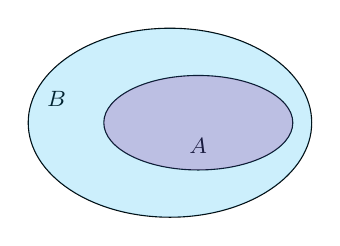
\begin{tikzpicture}[>=stealth,line join=round,line cap=round,font=\footnotesize,scale=.6]
			\coordinate (I)at(.4,1);
			\coordinate (M)at(1,1);
			\draw (.4,1) circle (3 and 2);
			\coordinate[label=center:$B$] (X)at(-2,1.5);
			\draw (1,1) circle (2 and 1);
			\coordinate[label=center:$A$] (X)at(1,.5);
			% \coordinate[label=center:Hình 1] (X)at(1,-1.5);
			\fill[cyan,opacity=.2] (I) ellipse (3 cm and 2 cm)--cycle;
			\fill[violet,opacity=.2] (M) ellipse (2 cm and 1 cm)--cycle;
	\end{tikzpicture}}
\end{khung4}
\begin{note}
	\immini {Giữa các tập hợp số quen thuộc (tập số tự nhiên, tập số nguyên, tập số hữu tỉ, tập số thực), ta có quan hệ bao hàm:
		$$\mathbb{N} \subset \mathbb{Z} \subset \mathbb{Q} \subset \mathbb{R}.$$}
	{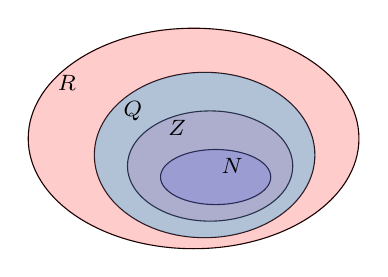
\begin{tikzpicture}[>=stealth,line join=round,line cap=round,font=\footnotesize,scale=.7]
			\path (1.3,1)coordinate[label=center:$$](M) (1.5,.7)coordinate[label=center:$$](N) (1.6,.5)coordinate[label=center:$$](P) (1.7,.3)coordinate[label=center:$$](Q);
			%(1.5,-1.5)coordinate[label=center](H);
			\draw (1.3,1) circle (3 and 2);
			\draw (1.5,.7) circle (2 and 1.5);
			\draw (1.6,.5) circle (1.5 and 1);
			\draw (1.7,.3) circle (1 and .5);
			\fill[red,opacity=.2] (M) ellipse (3 cm and 2 cm)--cycle;
			\fill[cyan,opacity=.3] (N) ellipse (2 cm and 1.5 cm)--cycle;
			\fill[violet,opacity=.1] (P) ellipse (1.5 cm and 1 cm)--cycle;
			\fill[blue,opacity=.1] (Q) ellipse (1 cm and .5 cm)--cycle;
			\coordinate[label=center:$\mathbb{R}$] (X)at(-1,2);
			\coordinate[label=center:$\mathbb{Q}$] (Q)at(0.2,1.5);
			\coordinate[label=center:$\mathbb{Z}$] (Z)at(1,1.2);
			\coordinate[label=center:$\mathbb{N}$] (N)at(2,.5);
	\end{tikzpicture}}
\end{note}
% \indam{Định nghĩa:}
\begin{khung4}{}
	Hai tập hợp $A$ và $B$ gọi là bằng nhau, kí hiệu $A=B$, nếu $A \subset B$ và $B \subset A$.
\end{khung4}
\begin{note}
	Nói cách khác, hai tập hợp $A$ và $B$ bằng nhau nếu mỗi phần tử của tập hợp này cũng là phần tử của tập hợp kia và ngược lại.
\end{note}
\newpage
\subsubsection{Một số tập con của tập hợp số thực}
Cho $a$ và $b$ là hai số thực với $a<b$.
\begin{center}
	\begin{tabular}{|c|c|c|}
		\hline
		Tên gọi và kí hiệu& Tập hợp& Biểu diễn trên trục số \tabularnewline
		\hline 
		Tập số thực $(-\infty;+\infty)$&$\mathbb{R}$&\begin{tikzpicture}[scale=1, font=\footnotesize, line join=round, line cap=round, >=stealth,baseline]
			\draw[->](0,0)->(5,0);
			\path
			(2.5,-0.1)coordinate[label=below:$0$](a)
			(2.5,0)coordinate[label=center:$|$](();
		\end{tikzpicture}
		\\\hline
		Đoạn $[a;b]$&$\left\lbrace x \in \mathbb{R} \ \middle|\ a\leq x \leq b\right\rbrace $&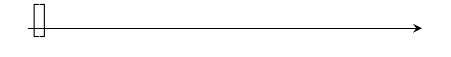
\begin{tikzpicture}[scale=1, font=\footnotesize, line join=round, line cap=round, >=stealth,baseline]
			\draw[->](0,0)->(5,0);
			\IntervalLR{0}{1.5}
			\def\skipInterval{0.5cm}
			\IntervalGRF{}{}{\big[}{a}
			\IntervalLR{3.5}{4.8}
			\def\skipInterval{0.5cm}
			\IntervalGRF{\big]}{b}{}{}
		\end{tikzpicture}
		\\\hline
		Khoảng $(a;b)$&$\left\{x\in\mathbb{R}\ \middle|\ a<x<b\right\}$
		&
		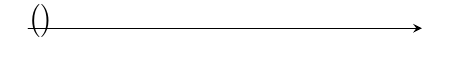
\begin{tikzpicture}[scale=1, font=\footnotesize, line join=round, line cap=round, >=stealth,baseline]
			\draw[->](0,0)->(5,0);
			\IntervalLR{0}{1.5}
			\def\skipInterval{0.5cm}
			\IntervalGRF{}{}{\big(}{a}
			\IntervalLR{3.5}{4.8}
			\def\skipInterval{0.5cm}
			\IntervalGRF{\big)}{b}{}{}
		\end{tikzpicture}
		\\\hline
		Nửa khoảng $[a;b)$&$\left\{x\in\mathbb{R}\ \middle|\ a\leq x<b\right\}$
		&
		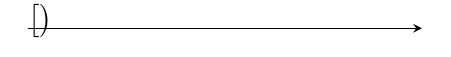
\begin{tikzpicture}[scale=1, font=\footnotesize, line join=round, line cap=round, >=stealth,baseline]
			\draw[->](0,0)->(5,0);
			\IntervalLR{0}{1.5}
			\def\skipInterval{0.5cm}
			\IntervalGRF{}{}{\big[}{a}
			\IntervalLR{3.5}{4.8}
			\def\skipInterval{0.5cm}
			\IntervalGRF{\big)}{b}{}{}
		\end{tikzpicture}
		\\\hline
		Nửa khoảng $(a;b]$&$\left\{x\in\mathbb{R}\ \middle|\ a<x\leq b\right\}$
		&
		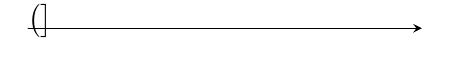
\begin{tikzpicture}[scale=1, font=\footnotesize, line join=round, line cap=round, >=stealth,baseline]
			\draw[->](0,0)->(5,0);
			\IntervalLR{0}{1.5}
			\def\skipInterval{0.5cm}
			\IntervalGRF{}{}{\big(}{a}
			\IntervalLR{3.5}{4.8}
			\def\skipInterval{0.5cm}
			\IntervalGRF{\big]}{b}{}{}
		\end{tikzpicture}
		\\\hline
		Nửa khoảng $(-\infty;a]$&$\left\{x\in\mathbb{R}\ \middle|\ x\leq a\right\}$ &
		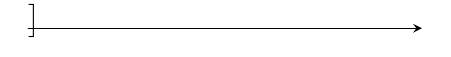
\begin{tikzpicture}[scale=1, font=\footnotesize, line join=round, line cap=round, >=stealth,baseline]
			\draw[->](0,0)->(5,0);
			\IntervalLR{0}{1.5}
			\IntervalLR{3.5}{4.8}
			\def\skipInterval{0.5cm}
			\IntervalGRF{\big]}{a}{}{}
		\end{tikzpicture}
		\\\hline
		Nửa khoảng $[a;+\infty)$&$\left\{x\in\mathbb{R}\ \middle|\ x\geq a\right\}$
		&
		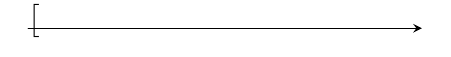
\begin{tikzpicture}[scale=1, font=\footnotesize, line join=round, line cap=round, >=stealth,baseline]
			\draw[->](0,0)->(5,0);
			\IntervalLR{0}{1.5}
			\def\skipInterval{0.5cm}
			\IntervalGRF{}{}{\big[}{a}
			\IntervalLR{3.5}{4.8}
		\end{tikzpicture}
		\\\hline
		Khoảng $(-\infty;a)$&$\left\{x\in\mathbb{R}\ \middle|\ x<a\right\}$ &
		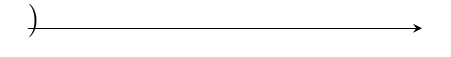
\begin{tikzpicture}[scale=1, font=\footnotesize, line join=round, line cap=round, >=stealth,baseline]
			\draw[->](0,0)->(5,0);
			\IntervalLR{0}{1.5}
			\IntervalLR{3.5}{4.8}
			\def\skipInterval{0.5cm}
			\IntervalGRF{\big)}{a}{}{}
		\end{tikzpicture}
		\\\hline
		Khoảng $(a;+\infty)$&$\left\{x\in\mathbb{R}\ \middle|\ x>a\right\}$
		&
		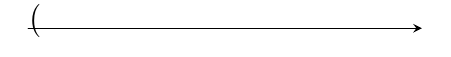
\begin{tikzpicture}[scale=1, font=\footnotesize, line join=round, line cap=round, >=stealth,baseline]
			\draw[->](0,0)->(5,0);
			\IntervalLR{0}{1.5}
			\def\skipInterval{0.5cm}
			\IntervalGRF{}{}{\big(}{a}
			\IntervalLR{4}{4.8}
		\end{tikzpicture}
		\\\hline
	\end{tabular}
\end{center}
Kí hiệu $-\infty$ đọc là \textbf{âm vô cực}, kí hiệu $+\infty$ đọc là \textbf{dương vô cực}.
\subsubsection{Hợp của hai tập hợp}
\begin{khung4}{}
	Cho hai tập hợp $A$ và $B$.\\
Tập hợp các phần tử thuộc $A$ hoặc thuộc $B$ gọi là \textbf{hợp} của hai tập hợp $A$ và $B$, kí hiệu $A \cup B$.\immini{
		\begin{itemize}
			\item $A \cup B = \{x \mid x \in A \text{ hoặc } x \in B\}$.
			\item $x \in A \cup B \Leftrightarrow \hoac{&	x \in A \\ & x \in B.}$
	\end{itemize}}
	{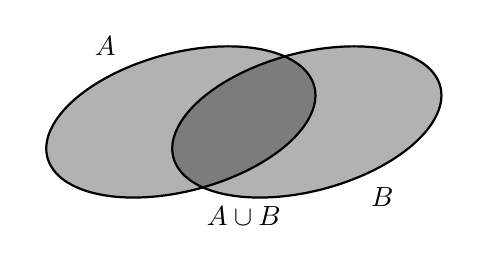
\begin{tikzpicture}[scale=.8]
			\fill[opacity=0.3,thick,cm={1, 0, 0.5, 0.8, (0,0)}] (-1,0) circle (2 and 1.5);
        \fill[opacity=0.3,thick,cm={1, 0, 0.5, 0.8, (0,0)}] (1,0) circle (2 and 1.5);
		\draw[thick,cm={1, 0, 0.5, 0.8, (0,0)}] (-1,0) circle (2 and 1.5);
        \draw[thick,cm={1, 0, 0.5, 0.8, (0,0)}] (1,0) circle (2 and 1.5);
			\node at (-2.2,1.2) {$A$};
			\node at (2.2,-1.2) {$B$};
			\node at (0,-1.5) {$A \cup B$};
	\end{tikzpicture}}
\end{khung4}
\subsubsection{Giao của hai tập hợp}
\begin{khung4}{}
Cho hai tập hợp $A$ và $B$.\\
Tập hợp các phần tử thuộc cả hai tập hợp $A$ và $B$ gọi là \textbf{giao} của hai tập hợp $A$ và $B$, kí hiệu $A \cap B$.
\immini{\begin{itemize}
		\item $A \cap B = \{x \mid x \in A \text{ và } x \in B\}$.
		\item $x \in A \cap B \Leftrightarrow \heva{& x \in A \\& x \in B.}$
\end{itemize}}
{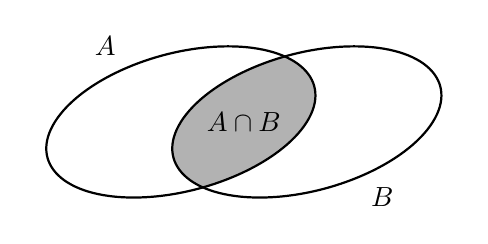
\begin{tikzpicture}[scale=.8]
		% Tô màu vùng giao
		\begin{scope}
			\clip[cm={1, 0, 0.5, 0.8, (0,0)}] (-1,0) circle (2 and 1.5);
			\fill[opacity=0.3,cm={1, 0, 0.5, 0.8, (0,0)}] (1,0) circle (2 and 1.5);
		\end{scope}
		\draw[thick,cm={1, 0, 0.5, 0.8, (0,0)}] (-1,0) circle (2 and 1.5);
        \draw[thick,cm={1, 0, 0.5, 0.8, (0,0)}] (1,0) circle (2 and 1.5);
			\node at (-2.2,1.2) {$A$};
			\node at (2.2,-1.2) {$B$};
			\node at (0,0) {$A \cap B$};
\end{tikzpicture}}
\end{khung4}
\begin{nx}
Nếu $A$ và $B$ không có phần tử chung, tức $A\cap B=\varnothing$ thì $n(A\cup B)=n(A)+n(B)$.
\end{nx}
\subsubsection{Hiệu của hai tập hợp, phần bù của tập con}
\begin{khung4}{}
	Tập hợp các phần tử thuộc $A$ nhưng không thuộc $B$ gọi là \textbf{hiệu} của $A$ và $B$, kí hiệu $A \setminus B$.
	\immini{
	\begin{itemize}
		\item $A \setminus B = \{x \mid x \in A \text{ và } x \notin B\}.$\
		\item $x \in A \setminus B \Leftrightarrow \heva{&x\in A\\& x\notin B.}$
	\end{itemize}	
}{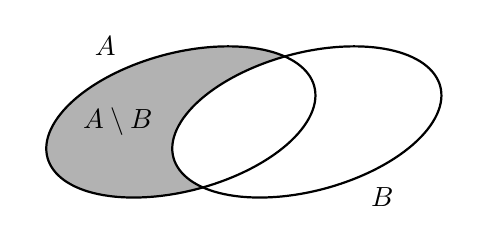
\begin{tikzpicture}[scale=.8]
		% Tô màu phần A \ B
		\begin{scope}
			\fill[opacity=0.3,cm={1, 0, 0.5, 0.8, (0,0)}] (-1,0) circle (2 and 1.5);
			\fill[cm={1, 0, 0.5, 0.8, (0,0)},white] (1,0) circle (2 and 1.5);
		\end{scope}
		\draw[thick,cm={1, 0, 0.5, 0.8, (0,0)}] (-1,0) circle (2 and 1.5);
        \draw[thick,cm={1, 0, 0.5, 0.8, (0,0)}] (1,0) circle (2 and 1.5);
			\node at (-2.2,1.2) {$A$};
			\node at (2.2,-1.2) {$B$};
			\node at (-2,0) {$A \setminus B$};
	\end{tikzpicture}	
}
\end{khung4}
\begin{khung4}{}
\immini{
\begin{itemize}
	\item Nếu $A \subset S$ thì hiệu $S \setminus A$ được gọi là \textbf{phần bù} của $A$ trong $S$, kí hiệu $\mathrm{C}_SA$.
	\end{itemize}
}{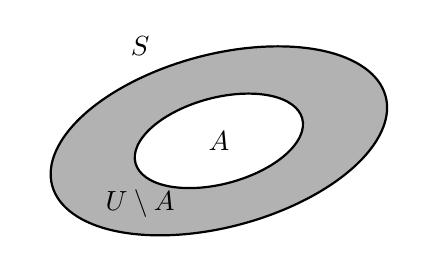
\begin{tikzpicture}
		\begin{scope}
			\fill[opacity=0.3,cm={1, 0, 0.5, 0.8, (0,0)}] (0,0) circle (2 and 1.5);
			\fill[cm={1, 0, 0.5, 0.8, (0,0)},white] (0,0) circle (1 and 0.75);
		\end{scope}
		\draw[thick,cm={1, 0, 0.5, 0.8, (0,0)}] (0,0) circle (2 and 1.5);
        \draw[thick,cm={1, 0, 0.5, 0.8, (0,0)}] (0,0) circle (1 and 0.75);
			\node at (-1,1.2) {$S$};
			\node at (0,0) {$A$};
			\node at (-1,-.8) {$U \setminus A$};
	\end{tikzpicture}}
\end{khung4}


\begin{note}
	Trong các chương sau, để tìm các tập hợp là giao, hợp, hiệu, phần bù của những tập con của tập số thực, ta thường vẽ sơ đồ trên trục số.
\end{note}
%-------------------------------------------
\subsection{PHÂN LOẠI VÀ PHƯƠNG PHÁP GIẢI TOÁN}
\begin{dang}{Xác định tập hợp}
	\begin{itemize}
		\item Kiểm tra các phần tử thuộc hay không thuộc tập hợp.
		\item Liệt kê các phần tử của tập hợp.
		\item Nêu tính chất đặc trưng của tập hợp.
	\end{itemize}
\end{dang}
\begin{vd}%[0D1H2-1]
	Viết các tập hợp sau đây dưới dang liệt kê các phần tử và tìm số phần tử của mỗi tập hợp đó:
	\begin{enumerate}
		\item Tập hợp $A$ các ước của $24$ \dotfill;
		\item Tập hợp $B$ gồm các chữ số trong số $1\,113\,305$\dotfill;
		\item $C=\{n \in \mathbb{N} \mid n~ \text{là bội của}~ 5 \text{và}~ n \leq 30\}$\dotfill;
		\item $D=\left\{x \in \mathbb{R} \mid x^2-2x+3=0\right\}$\dotfill.
	\end{enumerate}
\loigiai{
	\begin{enumerate}
		\item $A=\{-24;-12;-8;-6;-4;-3;-2;-1;1;2;3;4;6;8;12;24\}$, $n(A)=16$.
		\item $B=\{0;1;3;5\}$, $n(B)=4$.
		\item $C=\{0;5;10;15;20;25;30\}$, $n(C)=7$.
		\item $D=\varnothing$, $n(D)=0$. Do phương trình $x^2-2x+3=0$ vô nghiệm.
	\end{enumerate}
	}
\end{vd}
\begin{vd}%[0D1H2-1]
	Viết các tập hợp sau đây dưới dạng chỉ ra tính chất đặc trưng cho các phần tử:
	\begin{enumerate}
		\item $A=\{1; 3; 5; \ldots; 15\}$\dotfill;
		\item $B=\{0; 5; 10; 15; 20; \ldots\}$\dotfill;
		\item Tập hợp $C$ các nghiệm của bất phương trình $2x+5> 0$\dongcham{2}.
	\end{enumerate}
\loigiai{
	\begin{enumerate}
		\item $A=\{x\mid x~ \text{là số tự nhiên lẻ},\, x\geq 15\}$.
		\item $B=\{n \in \mathbb{N} \mid n~ \text{là bội của } 5\}$.
		\item $C=\{x\in \mathbb{R}\mid 2x+5>0\}$.
	\end{enumerate}
	}
\end{vd}
\begin{vd}
	Trong các tập hợp sau, tập hợp nào rỗng?
	\begin{enumEX}{1}
		\item $A=\left\{\left. x\in \mathbb{R}\right|x^2-x+1=0\right\}$\dongcham{2}
		\item $B=\left\{\left. x\in \mathbb{Q}\right|\right.x^2-4x+2\left. =0\right\}$\dongcham{2}
		\item $C=\left\{\left. x\in \mathbb{Z}\right|\right.6x^2-7x+1\left. =0\right\}$\dongcham{2}
		\item $D=\left\{\left. x\in \mathbb{Z}\right|\right.\left| x\right|<\left. 1\right\}$\dongcham{2}
	\end{enumEX}
\loigiai{
	\begin{enumEX}{1}
		\item Phương trình $x^2-x+1=0$ có $\Delta <0$ nên vô nghiệm. Do đó $A=\varnothing $.
		\item Phương trình $x^2-4x+2=0$ có hai nghiệm $x=2\pm \sqrt{2}\notin \mathbb{Q}$. Do đó $B=\varnothing $.
		\item Phương trình $6x^2-7x+1=0$ có nghiệm $x=1\in \mathbb{Z}$. Do đó $C\ne \varnothing $.
		\item Chọn $x=0\in \mathbb{Z},\left| 0\right|<1$. Do đó $D\ne \varnothing $.
	\end{enumEX}
	}
\end{vd}
\begin{dang}{Tập con và hai tập hợp bằng nhau}
	\begin{itemize}
		\item $\varnothing \subset A$  và $A \subset A$ với mọi tập hợp $A$
		\item Nếu tập hợp $A$ gồm $n$ phần tử thì tập $A$ có $2^n$ tập con.
	\end{itemize}
\end{dang}
\begin{vd}%[0D1H2-2]
	Trong mỗi cặp tập hợp sau đây, tập hợp nào là tập con của tập hợp còn lại? Chúng có bằng nhau không?
	\begin{enumerate}
		\item $A=\left\{-\sqrt{3}; \sqrt{3}\right\}$ và $B=\left\{x \in \mathbb{R} \mid x^2-3=0\right\}$\dongcham{2}
		\item $C$ là tập hợp các tam giác đều và $D$ là tập hợp các tam giác cân\dongcham{2}
		\item $E=\{x \in \mathbb{N} \mid x$ là ước của 12 $\}$ và $F=\{x \in \mathbb{N} \mid x$ là ước của 24 $\}$\dongcham{2}
	\end{enumerate}
\loigiai{
	\begin{enumerate}
		\item $A=B$.
		\item $C\subset D$ và $C\ne D$.
		\item $E\subset F$ và $E\ne F$.
	\end{enumerate}
	}
\end{vd}
\begin{vd}%[0D1H2-2]
	Viết tất cả các tập con của tập hợp $A=\{a; b\}$.\dongcham{2}
\loigiai{$\varnothing$, $\{a\}$, $\{b\}$, $\{a; b\}$. }
\end{vd}
\begin{vd}%[0D1B4-1]
	Cho hai tập hợp $A=\{a;b;c;d;e\}$ và $B=\{a;c;e;f\}$. Tìm tất cả các tập hợp $X$ sao cho $X\subset A$ và $X\subset B$.
	\dongcham{2}
\loigiai{
	Ta có $\left\{\begin{aligned}
	&X\subset A\\
	&X\subset B
	\end{aligned}\right. $, suy ra $X\subset \left(A\cap B\right)$. Mà $A\cap B=\{a;c;e\}$.\\
	Vậy các tập $X$ cần tìm là các tập con của tập $\{a;c;e\}$ nên gồm $\varnothing, \{a\}, \{c\}, \{e\}, \{a;c\}, \{a;e\}, \{c;e\}, \{a;c;e\}$.
	}
\end{vd}
\begin{vd}
	Cho hai tập hợp $A=\{1 ; a ; 5\}, B=\{a+2 ; 3 ; b\}$ với $a, b$ là các số thực. Biết rằng $A=B$, hãy xác định $a$ và $b$.
	\dongcham{2}
\loigiai{Vì $3 \in B$ và $A=B$ nên ta có $3 \in A=\{1 ; a ; 5\}$, do đó, $a=3$. Khi đó, $B=\{5 ; 3 ; b\}$.\\
	Vì $1 \in A$ và $A=B$ nên ta có $1 \in B=\{5 ; 3 ; b\}$. Suy ra, ta có $b=1$.\\
	Khi đó, $A=B=\{1 ; 3 ; 5\}$. Vậy các giá trị cần tìm là $a=3, b=1$.
	}
\end{vd}
\begin{dang}{Một số tập con của tập hợp số thực}
	Sử dụng phần \textbf{biểu diễn trên trục số} của phần \textbf{Một số tập con của tập hợp số thực} để giải quyết các bài toán.
\end{dang}
\begin{vd}%[0D1H2-3]
	Dùng các kí hiệu đoạn, khoảng, nửa khoảng để viết các tập hợp sau đây:
	\begin{listEX}[1]
		\item $\{x \in \mathbb{R} \mid-2< x < 3\}$\dotfill;
		\item $\{x \in \mathbb{R} \mid 1\leq x \leq 10\}$\dotfill;
		\item $\{x \in \mathbb{R} \mid-5< x \leq \sqrt{3}\}$\dotfill;
		\item $\{x \in \mathbb{R} \mid \pi \leq x < 4\}$\dotfill;
		\item $\left\{x \in \mathbb{R} \left\lvert x < \dfrac{1}{4}\right.\right\}$\dotfill;
		\item $\left\{x \in \mathbb{R} \left\lvert x \geq \dfrac{\pi}{2}\right.\right\}$\dotfill.
	\end{listEX}
\loigiai{
	\begin{listEX}[2]
		\item $\{x \in \mathbb{R} \mid-2< x < 3\}=(-2;3)$;
		\item $\{x \in \mathbb{R} \mid 1\leq x \leq 10\}=[1;10]$;
		\item $\{x \in \mathbb{R} \mid-5< x \leq \sqrt{3}\}=\left(-5;\sqrt{3}\,\right]$;
		\item $\{x \in \mathbb{R} \mid \pi \leq x < 4\}=[\pi;4)$;
		\item $\left\{x \in \mathbb{R} \left\lvert x < \dfrac{1}{4}\right.\right\}=\left(-\infty;\dfrac{1}{4}\right)$;
		\item $\left\{x \in \mathbb{R} \left\lvert x \geq \dfrac{\pi}{2}\right.\right\}=\left[\dfrac{\pi}{2};+\infty\right) $.
	\end{listEX}}
\end{vd}
\begin{dang}{Các phép toán trên tập hợp rời rạc}
% \textbf{Phương pháp giải:}
% \begin{itemize}
% 	\item \textbf{Tìm giao hai tập hợp $A$ và $B$:}
% 	\begin{itemize}
% 		\item So sánh từng phần tử của tập $A$ với các phần tử của tập $B$.
% 		\item Ghi lại các phần tử có mặt trong cả hai tập.
% 	\end{itemize}
% 	\item \textbf{Tìm hợp hai tập hợp $A$ và $B$:}
% 	\begin{itemize}
% 		\item Gộp tất cả phần tử của $A$ và $B$ lại thành một tập.
% 		\item Loại bỏ các phần tử trùng nhau.
% 	\end{itemize}
% \end{itemize}
% \begin{itemize}
% 	\item \textbf{Tìm hiệu hai tập hợp $A$ và $B$ ($A \setminus B$):}
% 	\begin{itemize}
% 		\item Lấy các phần tử thuộc $A$ nhưng không thuộc $B$.
% 		\item Ký hiệu: $A \setminus B = \{x \mid x \in A \text{ và } x \notin B\}$.
% 	\end{itemize}
% 	\item \textbf{Tìm phần bù của tập $A$ trong $U$:}
% 	\begin{itemize}
% 		\item Lấy các phần tử thuộc tập $U$ nhưng không thuộc $A$.
% 		\item Ký hiệu: $A' = U \setminus A = \{x \in U \mid x \notin A\}$.
% 	\end{itemize}
% \end{itemize}
\end{dang}
\begin{vd}%[Dự án KNTT lần 2, Nguyễn Tuấn]
	Cho hai tập hợp $A=\left\{0;1;2;3;4\right\}$ và $B=\left\{2;3;4;5;6\right\}$. Tìm các tập hợp $A\cup B, A\cap B, A\backslash B, B\backslash A$.
	\dongcham{4}
\loigiai{
	Ta có $A\backslash B=\left\{0;1\right\}$, $B\backslash A=\left\{5;6\right\}$, $A\cup B=\left\{0;1;2;3;4;5;6\right\}$, $A\cap B=\left\{2;3;4\right\}$.
	}
\end{vd}
\begin{vd}%[Dự án KNTT lần 2, Nguyễn Tuấn]
	Cho $A=\left\{x\in \left. \mathbb{N}\right|\right.x\le \left. 5\right\}$, $B=\left\{x\in \left. \mathbb{N}\right|\right.x=3k-1,k\in \mathbb{N},k\le \left. 3\right\}$. Xác định tập $A, B, A\cap B, A\cup B, A\backslash B, B\backslash A$.
	\dongcham{7}
\loigiai{
	Ta có $A=\left\{0;1;2;3;4;5\right\}$ và $B=\left\{-1;2;5;8\right\}$ nên
	\begin{enumEX}[+]{2}
		\item $A\cap B=\left\{2;5\right\}$,
		\item $A\cup B=\left\{-1;0;1;2;3;4;5;8\right\}$,
		\item $A\backslash B=\left\{0;1;3;4\right\}$,
		\item $B\backslash A=\left\{-1;8\right\}$.
	\end{enumEX}
	}
\end{vd}
\begin{vd}%[Dự án KNTT lần 2, Nguyễn Tuấn]
	Cho tập hợp $E=\left\{1;2;3;4;5;6;7;8;9\right\}$ và các tập hợp con $A=\left\{1;2;3;4\right\}$, $B=\left\{2;4;6;8\right\}$. Xác định $C_EA$, $C_EB$, $C_E\left(A\cup B\right)$, $C_EA\cap C_EB$.
	\dongcham{5}
\loigiai{\\
	Ta có $C_EA=E\backslash A=\left\{5;6;7;8;9\right\}$, $C_EB=E\backslash B=\left\{1;3;5;7;9\right\}$ suy ra $C_EA\cap C_EB=\left\{5;7;9\right\}$.\\
	$A\cup B=\left\{1;2;3;4;6;8\right\}$ suy ra $C_E\left(A\cup B\right)=E\backslash A\cup B=\left\{5;7;9\right\}$.
	}
\end{vd}
\begin{vd}%[Dự án KNTT lần 2, Nguyễn Tuấn]
	Xác định hai tập $A$, $B$ biết rằng
	$A\backslash B=\left\{1;5;7;8\right\}, B\backslash A=\left\{2;10\right\}, A\cap B=\left\{3;6;9\right\}$.
	\dongcham{3}
\loigiai{
	Theo định nghĩa về phép trừ hai tập hợp, ta có
	$\heva{
	& A\backslash B=\left\{1;5;7;8\right\}\subset A \\
	& A\backslash B=\left\{1;5;7;8\right\}\not\subset B \\}$ và $\heva{
	& B\backslash A=\left\{2;10\right\}\subset B \\
	& B\backslash A=\left\{2;10\right\}\not\subset A \\}$.\\
	Mặt khác, ta có $\heva{
	& A\cap B=\left\{3;6;9\right\}\subset A \\
	& A\cap B=\left\{3;6;9\right\}\subset B \\}$.\\
	Do đó suy ra, tập $A=\left(A\backslash B\right)\cup \left(A\cap B\right)=\left\{1;5;7;8;3;6;9\right\}$, $B=\left(B\backslash A\right)\cup \left(A\cap B\right)=\left\{2;10;3;6;9\right\}$.
	}
\end{vd}
\begin{vd}%[Dự án KNTT lần 2, Nguyễn Tuấn]
	Cho hai tập hợp $A=\left\{1;2\right\}$ và $B=\left\{1;2;3;4\right\}$. Tìm tất cả các tập hợp $X$ sao cho $A\cup X=B$.
	\dongcham{5}
\loigiai{
	Các tập $X$ cần tìm thỏa mãn yêu cầu bài toán là $\left\{3;4\right\}, \left\{1;3;4\right\}, \left\{2;3;4\right\}, \left\{1;2;3;4\right\}$.
	}
\end{vd}
\begin{dang}{Các phép toán trên tập hợp con của tập số thực}
	\textbf{Phương pháp giải:} Cho $A$, $B$ là hai tập con của tập số thực.
\begin{itemize}
	\item Để tìm $A \cap B$, ta làm như sau:
	\begin{itemize}
		\item Biểu diễn $A$, $B$ trên trục số; gạch bỏ phần không thuộc $A$, $B$.
		\item Phần không bị gạch là $A \cap B$.
	\end{itemize}
	\item Để tìm $A \cup B$, ta làm như sau:
	\begin{itemize}
		\item Biểu diễn $A$, $B$ trên trục số; tô đậm phần thuộc $A$, $B$.
		\item Phần tô đậm là $A \cup B$.
	\end{itemize}
	\item Để tìm $A \setminus B$, ta làm như sau:
\begin{itemize}
	\item Biểu diễn $A$, $B$ trên trục số; tô đậm phần thuộc $A$, gạch bỏ phần thuộc $B$.
	\item Phần tô đậm mà không bị gạch là $A \setminus B$.
\end{itemize}
\end{itemize}
Dựa vào các bước biểu diễn trên trục số để xác định các tập giao, hợp, hiệu theo thứ tự.
\end{dang}

\begin{vd}
Xác định các tập hợp sau và biểu diễn chúng lên trục số:
\begin{enumerate}
	\item $A=\left\{x \in \mathbb{R} \mid 1 \le x \le 3\right\}$\dotfill
	\item $B=\left\{x \in \mathbb{R} \mid x < -1\right\}$\dotfill 
	\item $C=\left\{x \in \mathbb{R} \mid x \ge 0 \right\}$\dotfill 
	\item $D=(0;4) \cap [2;5]$\dotfill
	\item $E=(0;4) \cap (-2;3]$\dotfill
	\item $F=(-1;+\infty) \cap (-\infty;5]$\dotfill
	\item $G=[-1;+\infty) \cap (-\infty;-1]$\dotfill
	\item $H=(0;4) \cup [2;5]$\dotfill
	\item $I=(-2;2) \cup [2;3)$\dotfill
	\item $J=(-3;1) \cup [2;+\infty)$\dotfill
	\item $K=(0;4) \cup [2;5]$\dotfill
	\item $L=(-\infty;4) \cup [1;+\infty)$\dotfill
	\item $M=(0;4) \setminus [2;5]$\dotfill
	\item $N=(-3;4] \setminus [4;5]$\dotfill
	\item $O=[-3;4] \setminus (-3;4)$\dotfill
	\item $P=[-1;3] \setminus (-2;5)$\dotfill
	\item $Q=[-1;3] \setminus (-1;+\infty)$\dotfill
	\item $R=(-\infty;1] \setminus (-1;+\infty)$\dotfill
	\item $S=\mathbb{R} \setminus (-1;+\infty)$\dotfill
	\item $T=C_{\mathbb{R}} A$, với $A=\left\{x \in \mathbb{R} \mid 1 \le x \le 3\right\}$\dotfill
	\item $U=C_{\mathbb{R}} B$, với $B=\left\{x \in \mathbb{R} \mid |x| < 2\right\}$\dotfill
	\item $V=\left\{x \in \mathbb{R} \mid x^2-3>0\right\}$\dotfill
	\item $W=\left\{x \in \mathbb{R} \mid 3x^2-1<0\right\}$\dotfill
	\item $X=\left\{x \in \mathbb{R} \mid 16-x^2 \ge 0 \right\}$\dotfill
	\item $Y=A \cap B$ với $A=\left\{x \in \mathbb{R} \mid x^2<4\right\}$ và $B=\left\{x \in \mathbb{R} \mid x^2 \ge 1\right\}$.\dongcham{2}
	\item $Z=A \cup (B \cap C)$ với $A=\left\{x \in \mathbb{R} \mid x^2<4\right\}$ và $B=\left\{x \in \mathbb{R} \mid x^2 \ge 1\right\}$ \\và $C=\left\{x \in \mathbb{R} \mid x \ge 0 \right\}$.\dongcham{3}
\end{enumerate}
	

\end{vd}
\begin{dang}{Các bài toán biện luận theo tham số}
\end{dang}
\begin{vd}%[Dự án KNTT lần 2, Nguyễn Tuấn]%[0D1B4-1]
	Cho hai tập hợp $A=(-3;5]$, $B=[a;+\infty)$. Tìm $a$ để
	\begin{listEX}[1]%số cột
		\item $A\cap B=[-2;5]$.\dotfill
		\item $A\cap B$ có đúng một phần tử.\dotfill
	\end{listEX}
\loigiai{ \begin{enumerate}
	\item Để $A\cap B=[-2;5]$ khi và chỉ khi $\left\{\begin{aligned}
	&a>-3\\
	&a=-2
	\end{aligned}\right. \Leftrightarrow a=-2$.\\
	Vậy $a=-2$ là giá trị cần tìm.
	\item Để $A\cap B$ có đúng một phần tử khi và chỉ khi $a=5$. Khi đó $A\cap B=\{5\}$.\\
	Vậy $a=5$ là giá trị cần tìm.
	\end{enumerate}
	}
\end{vd}
\begin{vd}%[Dự án KNTT lần 2, Nguyễn Tuấn]%[0D1K4-1]%
	Cho $A=(-\infty;m+1]$; $B=(-1;+\infty)$. Tìm tất cả giá trị của tham số $m$ để $A \cup B=\mathbb{R}$.
	\dongcham{2}
\loigiai{
	Để $A \cup B=\mathbb{R}$ thì $m+1 \geq -1 \Leftrightarrow m \geq -2$.}
\end{vd}
\begin{vd}%[Dự án KNTT lần 2, Nguyễn Tuấn]
	Cho số thực $a<0$ và hai tập hợp $A=\left(-\infty;9a\right)$, $B=\left(\dfrac{4}{a};+\infty \right)$. Tìm $a$ để $A\cap B\ne \varnothing $.
	\dongcham{3}
\loigiai{
	Để hai tập hợp $A$ và $B$ giao nhau khác rỗng khi và chỉ khi $9a>\dfrac{4}{a} \Leftrightarrow 9a^2<4$ (do $a<0$)
	$\Leftrightarrow a^2<\dfrac{4}{9} \Leftrightarrow -\dfrac{2}{3}<a<0$.\\
	Vậy $-\dfrac{2}{3}<a<0$ thỏa mãn yêu cầu bài toán.
	}
\end{vd}
\begin{vd}%[Dự án KNTT lần 2, Nguyễn Tuấn]%[0D1B4-1]
	Cho hai tập hợp $A=[-2;m]$, $B=(1;5]$. Tùy theo $m$, xác định tập $B\setminus A$.
	\dongcham{4}
\loigiai{
	Nếu $-2<m\leq 1$ thì $A\cap B=\varnothing $. Do đó $B\setminus A=B$.\\
	Nếu $1<m<5$ thì $A\cap B=(1;m)$. Do đó $B\setminus A=B\setminus (1;m)=[m;5]$.\\
	Nếu $m\ge 5$ thì $B\subset A$. Do đó $B\setminus A=\varnothing $.
	}
\end{vd}
\begin{dang}{Ứng dụng thực tế các phép toán tập hợp}
\begin{enumerate}
	\item \textbf{Vẽ biểu đồ Ven hỗ trợ tư duy trực quan:}
	\begin{itemize}
		\item Biểu đồ Ven giúp dễ dàng xác định số phần tử thuộc từng vùng.
		\item Luôn bắt đầu từ vùng giao nhau (nếu biết) rồi suy ra các vùng còn lại.
	\end{itemize}
	\item \textbf{Cẩn thận với dữ kiện ngôn ngữ:}
	\begin{itemize}
		\item \lq\lq Chỉ tham gia…\rq\rq $\rightarrow$ hiệu tập hợp.
		\item \lq\lq Ít nhất một…\rq\rq $\rightarrow$ hợp tập hợp.
		\item \lq\lq Cả hai…\rq\rq $\rightarrow$ giao tập hợp.
		\item \lq\lq Không tham gia…\rq\rq $\rightarrow$ phần bù hoặc hiệu với tập tổng quát.
	\end{itemize}
	\item \textbf{Không nhầm lẫn giữa số phần tử và tập hợp:}
	\begin{itemize}
		\item $A = \{ \text{các phần tử} \}$, còn $n(A)$ là số phần tử của $A$.
		\item Luôn ghi rõ khi tính $n(A)$, $n(A \cup B)$,$\ldots$ tránh bỏ qua bước.
	\end{itemize}
\end{enumerate}
\underline{Lưu ý:} \textbf{Đối với bài toán ba tập hợp:} (chỉ dùng trong trắc nghiệm)
	\[
	\begin{aligned}
		n(A \cup B \cup C) =&~ n(A) + n(B) + n(C)\\
		&- n(A \cap B) - n(B \cap C) - n(C \cap A)\\
		&+ n(A \cap B \cap C).
	\end{aligned}
	\]
\end{dang}
\begin{vd}%[Dự án KNTT lần 2, Nguyễn Tuấn]%[0D1B3-3]
	Trong kì thi học sinh giỏi cấp trường, lớp $10$C1 có $45$ học sinh trong đó có  $17$ bạn đạt học sinh giỏi Văn, $25$ bạn đạt học sinh giỏi Toán và $13$ bạn học sinh không đạt học sinh giỏi. Tìm số học sinh giỏi cả Văn và Toán của lớp $10$C1.
	\dongcham{5}
\loigiai{
	\immini{
	\begin{itemize}
		\item Gọi $A$, $B$ theo thứ tự là tập hợp các học sinh giỏi Văn và giỏi Toán của lớp.
		Theo đề ta có $n(A)=17$, $n(B)=25$, $n(A\cup B)= 45-13=32$.
		\item Số học sinh giỏi cả Văn và Toán là $$n(A \cap B )=n(A) + n(B) - n(A \cup B)=25+17-32=10.$$
	\end{itemize}
	}
	{	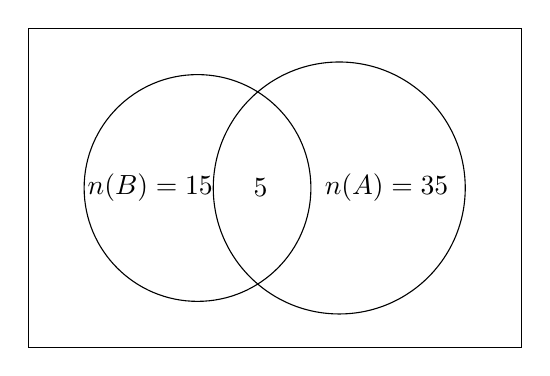
\begin{tikzpicture}[scale=.8]
	\def\radius{2cm}
	\coordinate (ceni);
	\coordinate[xshift=.9*\radius] (cenii);
	\draw (ceni) circle (.9*\radius);
	\draw (cenii) circle (\radius);
	\draw  ([xshift=-25pt,yshift=15pt]current bounding box.north west)
	rectangle ([xshift=25pt,yshift=-15]current bounding box.south east);
	\node[xshift=-.3*\radius] at (ceni) {$n(B)=15$};
	\node[xshift=.3*\radius] at (cenii) {$n(A)=35$};
	\node[xshift=.4*\radius] at (ceni) {$5$};
	\end{tikzpicture}}}
\end{vd}
\begin{vd}%[Dự án KNTT lần 2, Nguyễn Tuấn]%[0D1B3-3]
	Một lớp học có $ 50 $ học sinh trong đó có $ 30 $ em biết chơi bóng chuyền, $25$ em biết chơi bóng đá, $ 10 $ em biết chơi cả bóng đá và bóng chuyền. Hỏi có bao nhiêu em không biết chơi môn nào trong hai môn ở trên?
	\dongcham{5}
\loigiai{
	Gọi tập $A$ là tập hợp các học sinh biết chơi bóng chuyền.
	\\Tập $B$ là tập hợp các học sinh biết chơi bóng đá.
	\\Khi đó số học sinh biết chơi ít nhất một trong hai môn bóng chuyền hoặc bóng đá là
	$$n(A\cup B)=n(A)+n(B)-n(A\cap B)=30+25-10=45.$$
	Vậy số học sinh không biết chơi môn nào là $50-45=5$.
	}
\end{vd}
\begin{vd}%[Dự án KNTT lần 2, Nguyễn Tuấn]%[0D1B3-3]
	Lớp $10A$ có $15$ bạn thích môn Văn, $20$ bạn thích môn Toán. Trong số các bạn thích văn hoặc toán có $8$ bạn thích cả $2$ môn. Trong lớp vẫn còn $10$ bạn không thích môn nào trong $2$ môn Văn và Toán. Hỏi lớp $10A$ có bao nhiêu học sinh?
	\dongcham{5}
\loigiai{Ta sử dụng sơ đồ Ven.
	\begin{center}
		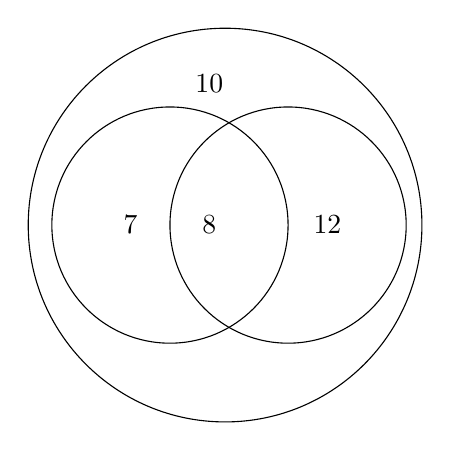
\begin{tikzpicture}
			\draw[] (0.7,0) circle ( 2.5cm);
			\draw[] (0,0) circle ( 1.5cm);
			\draw (1.5,0) circle ( 1.5 cm);
			\draw (-0.5,0) node {$7$};
			\draw (2,0) node {$12$};
			\draw (0.5,0) node {$8$};
			\draw (0.5,1.8) node {$10$};
		\end{tikzpicture}
	\end{center}
	\begin{itemize}
		\item Hình tròn lớn ngoài cùng thể hiện số học sinh cả lớp.\\
		Như vậy, ta có:\\
		\item	Số bạn chỉ thích Văn là $ 15-8=7$ (bạn).\\
		\item	Số bạn chỉ thích Toán là $20-8=12$ (bạn).\\
		\item	Số học sinh cả lớp là tổng các phần không giao nhau: $7+8+12+10=37$.
	\end{itemize}
	}
\end{vd}
\begin{vd}%[Dự án KNTT lần 2, Nguyễn Tuấn]%[0D1K3-3]
	Kết quả thi học kì một của một trường THPT có $48$ thí sinh giỏi môn Toán, $37$ thí sinh giỏi môn Vật Lí, $42$ thí sinh giỏi môn Văn. Biết rằng có $75$ thí sinh giỏi môn Toán hoặc môn Vật lí, $76$ thí sinh giỏi  môn Toán hoặc môn Văn, $66$ thí sinh giỏi môn Vật lí hoặc môn Văn và có $4$ thí sinh giỏi cả ba môn. Hỏi
	\begin{enumerate}
		\item có bao nhiêu học sinh chỉ giỏi 1 môn.
		\item có bao nhiêu học sinh chỉ giỏi 2 môn.
		\item có bao nhiêu học sinh giỏi ít nhất 1 môn.
	\end{enumerate}
	\dongcham{9}
\loigiai{
	\immini{
	Gọi $A$, $B$, $C$ theo thứ tự là tập hợp các học sinh giỏi Toán, giỏi Lí và giỏi Văn. Theo đề ta có
	\begin{itemize}
		\item Số học sinh giỏi Toán và Lí là $$n(A \cap B)=n(A)+n(B)-n(A\cup B)=48+37-75=10.$$
		\item Số học sinh giỏi Toán và Văn là $$n(A \cap C)=n(A)+|C|-|A\cup C|=48+42 - 76 = 14 .$$
		\item Số học sinh giỏi Lí và Văn là $$n(B \cap C)=n(B)+|C|-|B\cup C|= 42+37-66=13 .$$
		\item Số học sinh chỉ giỏi môn Toán $48-10-6-4=28$.
		\item Số học sinh chỉ giỏi môn Lí $37-6-4-9=18 $.
		\item Số học sinh chỉ giỏi môn Văn $42-10-9-4=19 $.
	\end{itemize}
	}{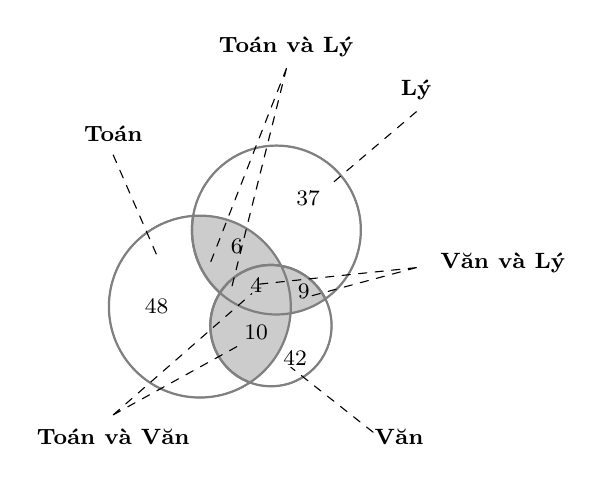
\begin{tikzpicture}[scale=0.55,>=stealth, font=\footnotesize, line join=round, line cap=round]
	\def\firstcircle{(0,0) circle (2.1cm)}
	\def\secondcircle{(45:2.5cm) circle (1.95cm)}
	\def\thirdcircle{(-15:1.7cm) circle (1.4cm)}
	\colorlet{circle edge}{black!50}
	\colorlet{circle area}{black!20}
	\tikzset{filled/.style={fill=circle area, draw=circle edge, thick},
	outline/.style={draw=circle edge, thick}}
	\draw \firstcircle;
	\draw \secondcircle;
	\draw \thirdcircle;
	\begin{scope}
		\clip \firstcircle;
		\fill[filled] \secondcircle;
	\end{scope}
	\begin{scope}
		\clip \firstcircle;
		\fill[filled] \thirdcircle;
	\end{scope}
	\begin{scope}
		\clip \secondcircle;
		\fill[filled] \thirdcircle;
	\end{scope}
	\node at (-1,0){48};
	\node at (2.2,-1.2){42};
	\node at (2.5,2.5){37};
	%
	\node at (0.85,1.4){6};
	\node at (1.3,0.5){4};
	\node at (1.3,-0.6){10};
	\node at (2.4,0.35){9};
	\draw[outline] \firstcircle
	\secondcircle  \thirdcircle;
	\node at (-2,4) {\textbf{Toán}};
	\node at (2,6) {\textbf{Toán và Lý}};
	\node at (5,5) {\textbf{Lý}};
	\node at (7,1) {\textbf{Văn và Lý}};
	\node at (4.6,-3) {\textbf{Văn}};
	\node at (-2,-3) {\textbf{Toán và Văn}};
	\draw[dashed] (-2,3.5) -- (-1,1.2)
	(2,5.5) -- (0.7,0.3)
	(2,5.5) -- (0.2,0.9)
	(5,4.5) -- (3,2.8)
	(5,0.9) -- (1.2,0.5)
	(5,0.9) -- (2.4,0.2)
	(4,-2.9) -- (2.1,-1.4)
	(-2,-2.5) -- (1.2,0.3)
	(-2,-2.5) -- (0.9,-0.9)	;
	\end{tikzpicture}}
	\begin{enumerate}
		\item Số học sinh chỉ giỏi đúng 1 môn là $28+18+19=65$.
		\item Số học sinh chỉ giỏi đúng 2 môn là $10+6+9=25$.
		\item Số học sinh giỏi ít nhất một môn là $65+25+4=94$.
	\end{enumerate}
	}
\end{vd}
%%%=============vd_3=============%%%
\begin{vd}%[Dự án KNTT lần 2, Nguyễn Tuấn]%[0D1V3-1]
	Lớp $10H$ có $37$ học sinh làm bài kiểm tra môn toán. Đề bài gồm có $3$ bài toán. Sau khi kiểm tra, cô giáo tổng hợp được kết quả như sau: có $20$ em giải được bài toán thứ nhất, $14$ em giải được bài toán thứ hai, $10$ em giải được bài toán thứ ba, $5$ em giải được bài toán thứ hai và thứ ba, $2$ em giải được bài toán thứ nhất và thứ hai, $6$ em giải được bài toán thứ nhất và thứ ba, chỉ có $1$ học sinh giải được cả ba bài toán. Hỏi lớp học đó có bao nhiêu học sinh không giải được bài toán nào?
	\dongcham{9}
\loigiai{
	Gọi tập $A$ là tập hợp học sinh giải được câu $1$. Tập $A$ có $20$ phần tử.\\
	Gọi tập $B$ là tập hợp học sinh giải được câu $2$. Tập $B$ có $14$ phần tử.\\
	Gọi tập $C$ là tập hợp học sinh giải được câu $3$. Tập $C$ có $10$ phần tử.\\
	Gọi tập $A\cap B$ là tập hợp học sinh giải được câu $1$ và câu $2$. Tập $A\cap B$ có $2$ phần tử.\\
	Gọi tập $B\cap C$ là tập hợp học sinh giải được câu $2$ và câu $3$. Tập $B\cap C$ có $5$ phần tử.\\
	Gọi tập $A\cap C$ là tập hợp học sinh giải được câu $1$ và câu $3$. Tập $A\cap C$ có $6$ phần tử.\\
	Gọi tập $A\cap B\cap C$ là tập hợp học sinh giải được cả $3$ câu. Tập $A\cap B\cap C$ có $1$ phần tử.\\
	Áp dụng nguyên lý bù trừ ta có
	\begin{eqnarray*}
		&n(A\cup B\cup C)&=n(A)+n(B)+n(C)-n(A
		\cap B)-n(B\cap C)-n(A\cap C)+n(A\cap B\cap C)\\
		&&=20+14+10-2-5-6+1\\
		&&=32.
	\end{eqnarray*}
	Số học sinh không giải được bài toán nào là $37-32=5$ (học sinh).
	}
\end{vd}
%-------------------------------------------
\subsection{BÀI TẬP TỰ LUYỆN}
\baitaptl

\setcounter{bt}{0}
\begin{bt}%[0D1H2-2]
	Cho ba tập hợp $A=\{2;5\}$, $B=\{5;x\}$ và $C=\{x;y;5\}$. Tìm các giá trị của $x$, $y$ sao cho $A=B=C$.
	\loigiai
	{
	Để $A=B \Leftrightarrow x=2$.\\
	Với $x=2$, suy ra $C=\{2;y;5\}$. Khi đó $\left\{\begin{aligned}
	&\{2;y;5\}\subset \{2;5\}\\
	&\{x;y;5\}\subset \{5;2\}
	\end{aligned}\right. $ hay $\left\{\begin{aligned}
	&A\subset C\\
	&B\subset C
	\end{aligned}\right. $.\\
	Do đó để $A=B=C$ khi và chỉ khi $\left\{\begin{aligned}
	&C\subset A\\
	&C\subset B
	\end{aligned}\right. \Leftrightarrow y=2$ hoặc $y=5$.\\
	Vậy $(x;y)=(2;2)$ hoặc $(x;y)=(2;5)$ thỏa mãn yêu cầu bài toán.
	}
\end{bt}
\begin{bt}%[0D1H3-1]%[Dự án KNTT lần 2, Nguyễn Tuấn]
	Cho các tập hợp sau:
	\begin{itemize}
		\item [] $A=\left\{\left. x\in \mathbb{Z}\right|-1\le x<6\right\}$;
		\item [] $B=\left\{\left. x\in \mathbb{Q}\right|\left(1-3x\right)\left({x}^4-3x^2+2\right)=0\right\}$;
		\item [] $C=\left\{0;1;2;3;4;5;6\right\}$.
	\end{itemize}
	\begin{enumEX}{1}
		\item Viết các tập hợp $A$, $B$ dưới dạng liệt kê các phần tử.
		\item Tìm $A\cap B$, $A\cup B$, $A\backslash B$, ${C}_{B\cup A}A\cap B$.
		\item Chứng minh rằng $A\cap (B\cup C)=A.$
	\end{enumEX}
\loigiai{
	\begin{enumerate}
		\item Ta có $A=\left\{-1; 0; 1; 2; 3; 4; 5\right\}$, $B=\left\{-1;\dfrac{1}{3};1\right\}$.
		\item Suy ra $A\cap B=\left\{-1;1\right\}$, $A\cup B=\left\{-1;0;\dfrac{1}{3};1;2;3;4;5\right\}$, $A\backslash B=\left\{0;2;3;4;5\right\}$ và ${C}_{B\cup A}\left(A\cap B\right)=\left\{0;\dfrac{1}{3};2;3;4;5\right\}$.
		\item Ta có $B\cup C=\left\{-1;0;1/3;1;2;3;4;5;6\right\}$ suy ra $A\cap \left(B\cup C\right)=\left\{-1;0;1;2;3;4;5\right\}=A$.
	\end{enumerate}
	}
\end{bt}
\begin{bt}%[0D1H3-1]%[Dự án KNTT lần 2, Nguyễn Tuấn]
	Cho các tập hợp sau:
	\begin{itemize}
		\item $A=\left\{\left. x\in \mathbb{R}\right|\left({x}^2+7x+6\right)\left(x^2-4\right)=0\right\}$
		\item $B=\left\{\left. x\in \mathbb{N}\right|2x\le 8\right\}$
		\item $C=\left\{\left. 2x+1\right|x\in \mathbb{Z}\right.$ và $\left.-2\le x\le 4\right\}$.
	\end{itemize}
	\begin{enumEX}{1}
		\item Hãy viết lại các tập hợp $A$, $B$, $ C$ dưới dạng liệt kê các phần tử.
		\item Tìm $A\cup B$, $A\cap B$, $B\backslash C$, ${C}_{A\cup B}\left(B\backslash C\right)$.
		\item Tìm $\left(A\cup C\right)\backslash B$.
	\end{enumEX}
\loigiai{
	\begin{enumerate}
		\item Phương trình $\left({x}^2+7x+6\right)\left(x^2-4\right)=0\Leftrightarrow \hoac{
		& x^2+7x+6=0 \\
		& x^2-4=0 \\}\Leftrightarrow \hoac{
		& x=-1\vee x=-6 \\
		& x=-2\vee x=2.}$\\
		Vậy $A=\left\{-6;-2;-1;2\right\}$.\\
		Ta có $\heva{
		& x\in \mathbb{N} \\
		& 2x\le 8 \\}\Leftrightarrow \heva{
		& x\in \mathbb{N} \\
		& x\le 4 \\}\Leftrightarrow x\in \left\{0,1,2,3,4\right\}$. Vậy $B=\left\{0;1;2;3;4\right\}$.\\
		Ta có $\heva{
		& x\in \mathbb{Z} \\
		&-2\le x\le 4 \\}\Leftrightarrow x\in \left\{-2,-1,0,1,2,3,4\right\}$. Vậy $C=\left\{-3;-1;1;3;5;7;9\right\}$.
		\item Suy ra $A\cup B=\left\{-6;-2;-1;0;1;2;3;4\right\}$, $A\cap B=\left\{2\right\}$, $B\backslash C=\left\{0;2;4\right\}$,
		${C}_{A\cup B}\left(B\backslash C\right)=\left(A\cup B\right)\backslash \left(B\backslash C\right)=\left\{-6;-2;-1;1;3\right\}$.
		\item Ta có $A\cup C=\left\{-6;-3;-2;-1;1;2;3;5;7;9\right\}$. Suy ra $(A\cup C)\backslash B=\left\{-6;-3;-2;-1;5;7;9\right\}$.
	\end{enumerate}
	}
\end{bt}
\begin{bt}%[Dự án KNTT lần 2, Nguyễn Tuấn]%[0D1H3-4]
	Cho đoạn $A=[-5;1]$ và khoảng $B=(-3;2)$. Xác định $A\cup B$, $A\cap B$, $A\setminus B$, $C_{\mathbb{R}}B$.
\loigiai{
	Ta có
	\begin{itemize}
		\item $A\cup B=[-5;2)$.
		\item $A\cap B=(-3;1]$.
		\item $A\setminus B=[-5;-3]$.
		\item $C_{\mathbb{R}}B=\mathbb{R}\setminus B=(-\infty;-3]\cup [2;+\infty)$.
	\end{itemize}
	}
\end{bt}
\begin{bt}%[Dự án KNTT lần 2, Nguyễn Tuấn]%[0D1H3-4]
	Cho các tập hợp $A=\left\{x\in \mathbb{R}\big|x^2\leq 4\right\}$, $B=\left\{x\in \mathbb{R}\big|x<1\right\}$. Viết các tập hợp sau đây $A\cup B$, $A\cap B$, $A\setminus B$, $ C_{\mathbb{R}}B$ dưới dạng các khoảng, nửa khoảng, đoạn.
\loigiai{
	Ta có $A=[-2;2]$ và $B=(-\infty;1)$, suy ra
	\begin{itemize}
		\item $A\cup B=[-2;2]\cup (-\infty;1)=(-\infty;2]$.
		\item $A\cap B=[-2;2]\cap (-\infty;1)=[-2;1)$.
		\item $A\setminus B=[-2;2]\setminus (-\infty;1)=[1;2]$.
		\item $C_{\mathbb{R}}B=[1;+\infty)$.
	\end{itemize}
	}
\end{bt}
\begin{bt}%[Dự án KNTT lần 2, Nguyễn Tuấn]%[0D1H3-3]
	Cho các nửa khoảng $A=(a;a+1]$, $B=[b;b+2)$.
	\begin{listEX}[1]
		\item Gọi $C=A\cup B$. Với điều kiện nào của $a, b$ thì $C$ là một đoạn. Tính độ dài của $C$ khi đó.
		\item Gọi $C=A\cap B$. Với điều kiện nào của $a, b$ thì $C$ là một đoạn. Tính độ dài của $C$ khi đó.
	\end{listEX}
\loigiai{
	Điều kiện: $a, b\in \mathbb{R}$.
	\begin{listEX}[1]
		\item Để $C=A\cup B$ là một đoạn khi và chỉ khi\\
		$b\leq a<b+2\leq a+1 \Leftrightarrow \left\{\begin{aligned}
		&b\leq a<b+2\\
		&b+2\leq a+1
		\end{aligned}\right. \Leftrightarrow \left\{\begin{aligned}
		&b\leq a<b+2\\
		&b+1\leq a
		\end{aligned}\right. \Leftrightarrow b+1\leq a<b+2$.\\
		Khi đó $C=[b;b+2)\cup (a;a+1]=[b; a+1]$ là đoạn có độ dài $a-b+1$.
		\item Để $C=A\cap B$ là một đoạn khi và chỉ khi\\
		$a<b<a+1<b+2 \Leftrightarrow \left\{\begin{aligned}
		&a<b\\
		&b<a+1<b+2
		\end{aligned}\right. \Leftrightarrow \left\{\begin{aligned}
		&a<b\\
		&b-1<a<b+1
		\end{aligned}\right. \Leftrightarrow b-1<a<b$.\\
		Khi đó $C=[b;b+2)\cap (a;a+1]=[b; a+1]$ là đoạn có độ dài $a-b+1$.
	\end{listEX}}
\end{bt}
\begin{bt}%[Dự án KNTT lần 2, Nguyễn Tuấn]%[0D1H3-3]
	Cho hai tập hợp $A=[a;a+2]$, $B=[b;b+1]$. Tìm điều kiện của $a$, $b$ để $A\cap B\ne \varnothing $.
\loigiai{
	Ta xét trường hợp $A\cap B=\varnothing $.\\
	Để $A\cap B=\varnothing $ khi và chỉ khi $\left[\begin{aligned}
	&a+2<b\\
	&b+1<a
	\end{aligned}\right. \Leftrightarrow \left[\begin{aligned}
	&a<b-2\\
	&a>b+1.
	\end{aligned}\right. $\\
	Từ đó suy ra điều kiện để $A\cap B\ne \varnothing $ là $b-2\leq a\leq b+1$.
	}
\end{bt}
\begin{bt}%[0D1H3-3]%[Dự án KNTT lần 2, Nguyễn Tuấn]
	Cho hai tập hợp $A=\left[2;m+1\right]$ và $B=\left[\dfrac{1}{2};+\infty \right)$. Tìm $m$ để $A\cap B$ chỉ có đúng 1 phần tử.
\loigiai{
	Điều kiện: $2<m+1\Leftrightarrow m>1$.\\
	Để $A\cap B$ chỉ có đúng 1 phần tử khi và chỉ khi $m+1=\dfrac{1}{2}\Leftrightarrow m=-\dfrac{1}{2}$: không thỏa mãn điều kiện.\\
	Vậy không tồn tại giá trị của $m$ để thỏa mãn yêu cầu bài toán.
	}
\end{bt}
\begin{bt}%[Dự án KNTT lần 2, Nguyễn Tuấn]%[0D1V3-2]
	Hãy xác định các tập $A$ và $B$ thỏa mãn đồng thời các điều kiện sau:
	\begin{enumerate}
		\item $A\cap B=\{1; 2; 3\}$, $A\setminus B=\{4; 5\}$ và $B\setminus A=\{6; 9\}$.
		\item $A\cap B=\{0; 1; 2; 3; 4\}$, $A\setminus B=\{-3;-2\}$ và $B\setminus A=\{6; 9; 10\}$.
		\item $A\setminus B=\{1; 5; 7; 8\}$, $A\cap B=\{3; 6; 9\}$ và $A\cup B=\{x \in \mathbb{N} \mid 0< x \leq 10\}$.
	\end{enumerate}
\loigiai{
	\begin{enumerate}
		\item Ta có $A=(A\cap B)\cup (A\setminus B)=\{1;2;3;4;5\}$.\\
		$B=(A\cap B)\cup (B\setminus A)=\{1;2;3;6;9\}$.
		\item Ta có $A=(A\cap B)\cup (A\setminus B)=\{-3;-2;0; 1; 2; 3; 4\}$.\\
		$B=(A\cap B)\cup (B\setminus A)=\{0; 1; 2; 3; 4;6; 9; 10\}$.
		\item Ta có $A\cup B=\{1;2;3;4;5;6;7;8;9;10\}$.\\
		$A=(A\cap B)\cup (A\setminus B)=\{1;3;5;6;7;8;9\}$.\\
		Ta có $B=(A\cup B)\setminus(A\setminus B)=\{2;3;4;6;9;10\}$.
	\end{enumerate}
	}
\end{bt}
\begin{bt}%[Dự án KNTT lần 2, Nguyễn Tuấn]%[0D1V3-4]
	Cho hai tập hợp $A = (3m-1; 3m+7)$ và $B = (-1; 1)$, với $m$ là tham số.
	\begin{enumerate}
		\item Tìm tất cả các tham số $m$ để $B \subset A$.
		\item Tìm tất cả các tham số $m$ để $A \cap B = \varnothing$.
	\end{enumerate}
\loigiai{
	\begin{enumerate}
		\item
		Để $B \subset A$, khoảng $(-1; 1)$ phải nằm hoàn toàn bên trong khoảng $(3m-1; 3m+7)$.\\
		Điều này tương đương với hệ bất phương trình
		$$\heva{& 3m - 1 \le -1 \\ & 3m + 7 \ge 1} \Leftrightarrow \heva{& 3m \le 0 \\ & 3m \ge -6} \Leftrightarrow \heva{& m \le 0 \\ & m \ge -2.}$$
		Vậy để $B \subset A$ thì $-2 \le m \le 0$.
		\item
		Để $A \cap B = \varnothing$, có các trường hợp sau\\
		\textbf{Trường hợp 1:} $3m - 1 \ge 1  \Leftrightarrow m \ge \dfrac{2}{3}$.\\
		\textbf{Trường hợp 2:} $3m + 7 \le -1  \Leftrightarrow m \le -\dfrac{8}{3}$.\\
		Kết hợp cả hai trường hợp, các giá trị của $m$ để $A \cap B = \varnothing$ là $m \ge \dfrac{2}{3}$ hoặc $m \le -\dfrac{8}{3}$.
	\end{enumerate}
	}
\end{bt}
\begin{bt}%[Dự án KNTT lần 2, Nguyễn Tuấn]%[0D1B3-3]
	Một lớp có $40$ học sinh, mỗi học sinh đều đăng ký chơi ít nhất $1$ trong $2$ môn thể thao là bóng đá hoặc cầu lông. Có $30$ học sinh có đăng ký môn bóng đá, $25$ học sinh có đăng ký môn cầu lông. Hỏi có bao nhiêu em đăng ký cả $2$ môn.
\loigiai{
	Gọi $A$ là tập hợp các học sinh đăng kí chơi bóng đá, $B$ là tập học sinh đăng kí chơi cầu lông thì $A\cap B$ là tập hợp các học sinh đăng kí chơi cả hai môn.\\
	Vậy số học sinh đăng kí chơi cả hai môn là
	$n(A\cap B)=n(A)+n(B)-n(A\cup B)=30+25-40=15$. }
\end{bt}
\begin{bt}%[Dự án KNTT lần 2, Nguyễn Tuấn]%[0D1B3-3]
	Mỗi học sinh của lớp $10A$ đều chơi bóng đá hoặc bóng chuyền. Biết rằng có $25$ bạn chơi bóng đá, $20$ bạn chơi bóng chuyền và $10$ bạn chơi cả $2$ môn thể thao. Hỏi lớp $10A$ có bao nhiêu học sinh.
\loigiai{
	Gọi $A$ là tập hợp các học sinh chơi bóng đá, $B$ là tập các học sinh chơi bóng chuyền. Do đó $A\cap B$ là tập các học sinh chơi cả hai môn.\\
	Theo đề $n(A)=25$, $n(B)=20$, $|A \cap B| =10$.\\
	Vậy số học sinh cả lớp là $|A \cup B| =n(A)+n(B)-n(A\cap B)=25+20-10=35$.}
\end{bt}
\begin{bt}%[Dự án KNTT lần 2, Nguyễn Tuấn]%[0D1B3-3]
	Lớp 10A có $45$ học sinh, có $15$ học sinh giỏi và $20$ học sinh xếp hạnh kiểm tốt, trong đó có $10$ bạn vừa học giỏi vừa xếp hạnh kiểm tốt. Các học sinh được học sinh giỏi hoặc hạnh kiểm tốt đều được khen thưởng. Số học sinh được khen thưởng của lớp 10A là là bao nhiêu?
\loigiai{
	Gọi $A$ là tập hợp các học sinh giỏi,
	$B$ là tập hợp các học sinh xếp hạnh kiểm tốt.\\
	Khi đó số học sinh được khen thưởng là $n(A\cup B)$.\\
	Vậy số học sinh được khen thưởng là
	$n(A\cup B)=n(A)+n(B)-n(A\cap B)=15+20-10=25.$
	}
\end{bt}
\begin{bt}%[Dự án KNTT lần 2, Nguyễn Tuấn]%[0D1K3-3]
	Một nhóm học sinh giỏi các bộ môn: Anh, Toán, Văn. Có $ 18 $ em giỏi Văn, $ 10 $ em giỏi Anh, $ 12 $ em giỏi Toán, $ 3 $ em giỏi Văn và Toán, $ 4 $ em giỏi Toán và Anh, $ 5 $ em giỏi Văn và Anh, $ 2 $ em giỏi cả ba môn. Hỏi nhóm đó có bao nhiêu em?
\loigiai{
	\immini
	{Ký hiệu $ A $ là tập hợp những học sinh giỏi Anh,\\
	$ T $ là tập hợp những học sinh giỏi Toán,\\
	$ V $ là tập hợp những học sinh giỏi Văn.\\
	$\bullet$ $|V|=18,\; n(A)=10,\; |T|=12$,\\
	$\bullet$ $|T \cap V|=3,\; |T \cap A|=4,\; |V \cap A|=5, |A \cap B \cap C|=2$.\\
	Số học sinh của nhóm là
	\begin{eqnarray*}
		|V \cup A \cup T|&=&|V|+n(A)+|T|-|V \cap A|-|T \cap A|-|T \cap V|+|A \cap B \cap C|\\
		&=&18+10+12-(3+4+5)+2=30.
	\end{eqnarray*}
	Vậy nhóm đó có $ 30 $ em.
	}
	{
	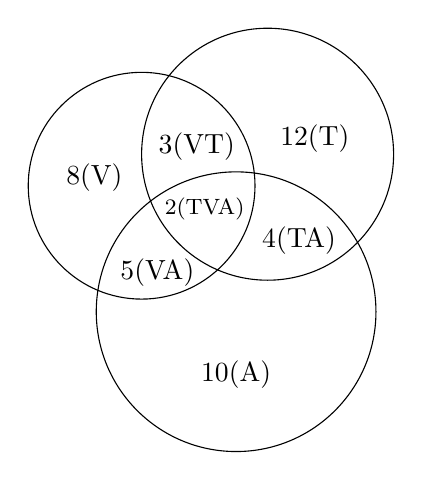
\begin{tikzpicture}[scale=.8]
		\def\radius{2cm}
		\coordinate (ceni);
		\coordinate[xshift=.8*\radius, yshift=.2*\radius] (cenii);
		\coordinate[xshift=.6*\radius,yshift=-.8*\radius] (ceniii);
		\draw (ceni) circle (.9*\radius);
		\draw (cenii) circle (\radius);
		\draw (ceniii) circle (1.11*\radius);
		\node[xshift=-.3*\radius, yshift=.05*\radius] at (ceni) {$8$(V)};
		\node[xshift=.35*\radius, yshift=.25*\radius] at (ceni) {$3$(VT)};
		\node[xshift=.1*\radius, yshift=-.55*\radius] at (ceni) {$5$(VA)};
		\node[xshift=.4*\radius, yshift=-.15*\radius] at (ceni) {{\footnotesize $2$(TVA)}};
		\node[xshift=.2*\radius, yshift=-.55*\radius] at (cenii) {$4$(TA)};
		\node[xshift=1.1*\radius,yshift=.3*\radius] at (ceni) {$12$(T)};
		\node[yshift=-.4*\radius] at (ceniii) {$10$(A)};
	\end{tikzpicture}
	}
	}
\end{bt}

\baitaptn
%-------------Trắc nghiệm nhiều lựa chọn
\TN
\setcounter{ex}{0}
\Opensolutionfile{ans}[ans/ans-c1b1-lc]
\begin{ex}%[0D1H2-1]
	Cho tập hợp $A = \{n \in \mathbb{N} \mid 3 \le n \le 10\}$. Dạng liệt kê của tập hợp $A$ là
	\choice
	{$A = \{3;4;5;6;7;8;9\}$}
	{$A = \{4;5;6;7;8;9;10\}$}
	{$A = \{4;5;6;7;8;9\}$}
	{\True $A = \{3;4;5;6;7;8;9;10\}$}
\loigiai{
	Với $n \in \mathbb{N}$ và $3 \le n \le 10$ thì $n \in \{3;4;5;6;7;8;9;10\}$ }
\end{ex}
\begin{ex}%[0D1H2-2]
	Cho tập hợp $A = \{n \in \mathbb{Z} \mid -2 < n \le 5\}$. Tập hợp $A$ bằng tập hợp nào sau đây?
	\choice
	{$M = \{-1; 0; 1;2;3;4 \}$}
	{$N = \{-1; 1;2;3;4; 5 \}$}
	{\True $P = \{-1;0;1;2;3;4;5 \}$}
	{$Q = \{-2;-1; 0; 1;2;3;4 \}$}
\loigiai{
	Với $n \in \mathbb{Z}$ và $-2 < n \le 5$ thì $n \in \{-1;0;1;2;3;4;5\}$ }
\end{ex}
\begin{ex}%[0D1H2-2]
	Tập hợp $A = \left\{1;2;3\right\}$ có bao nhiêu tập con gồm hai phần tử?
	\choice
	{$1$}
	{$2$}
	{\True $3$}
	{$4$}
\loigiai{
	Các tập con có hai phần tử của $A$ là $\{1;2\}$; $\{1;3\}$; $\{2;3\}$.\\
	Vậy có tất cả $3$ tập con thỏa yêu cầu.}
\end{ex}
\begin{ex}%[0D1V2-2]
	Có bao nhiêu tập hợp $X$ thoả mãn điều kiện $\left\{a; b\right\}\subset X \subset \left\{a;b;c;d;e\right\}$?
	\choice
	{$2$}
	{$4$}
	{\True $8$}
	{$10$}
\loigiai{Từ điều kiện $\left\{a; b\right\}\subset X \subset \left\{a;b;c;d;e\right\}$ ta suy ra $X$ tối thiểu phải chứa các phần tử $a, b$ và chỉ có thể thêm các phần tử $c, d, e$ nên chọn $X$ là một trong các tập hợp sau:
	$$\left\{a; b \right\},\quad \left\{a; b; c \right\},\quad \left\{a; b; d \right\},\quad \left\{a; b; e \right\},\quad \left\{a; b; c; d \right\},\quad \left\{a; b; d; e \right\},\quad \left\{a; b; e; c \right\},\quad \left\{a; b; c; d; e \right\}.$$
	Vậy có $8$ tâp hợp $X$ thoả mãn yêu cầu bài toán.}
\end{ex}
\begin{ex}%[0D1N2-3]
	Sử dụng các kí hiệu đoạn, khoảng, nửa khoảng đế viết tập hợp $A=\{x \in \mathbb{R} \mid x \leq 2\}$ là
	\choice
	{$A=(-\infty; 2)$}
	{\True $A=(-\infty; 2]$}
	{$A=[2;+\infty)$}
	{$A=(2;+\infty)$}
\loigiai{
	Ta có $A=(-\infty; 2]$.
	}
\end{ex}
\begin{ex}%[0D1H2-2]
	Cho tập hợp $A=\{1; 2; 5; 7\}$ và $B=\{1; 2; 3\}$. Có tất cả bao nhiêu tập $X$ thỏa mãn $X\subset A$ và $X\subset B$?
	\choice
	{$5$}
	{\True $4$}
	{$3$}
	{$6$}
\loigiai{
	Vì $X$ thỏa mãn $X\subset A$ và $X\subset B$ nên $X\subset A\cap B=\{1;2\}$.\\
	Do $A\cap B$ có $2$ phần tử nên có $2^2=4$ tập con.
	}
\end{ex}
\begin{ex}%[Dự án KNTT lần 2, Nguyễn Tuấn]%[0D1N3-1]
	Cho hai tập hợp $A=\{0 ; 1 ; 2 ; 3 ; 4 ; 5\}$ và $B=\{2 ; 4 ; 6 ; 7\}$. Tập $A \cap B$ là
	\choice
	{$\{2 ; 4 ; 6 ; 7\}$}
	{\True $\{2 ; 4\}$}
	{$\{2 ; 4 ; 6\}$}
	{$\{0 ; 1 ; 3 ; 5\}$}
\loigiai{
	Ta có $A \cap B = \{2 ; 4\}$.
	}
\end{ex}
\begin{ex}%[Dự án KNTT lần 2, Nguyễn Tuấn]%[0D1N3-1]
	Cho hai tập hợp $A=\{1 ; 2 ; 4 ; 7 ; 9\}$ và $B=\{-1 ; 0 ; 7 ; 10\}$. Tập hợp $A \cup B$ có tất cả bao nhiêu phần tử?
	\choice
	{$9$}
	{$7$}
	{\True $8$}
	{$10$}
\loigiai{
	Ta có $A \cup B = \{-1;1;0 ; 2 ; 4 ; 7 ; 9 ;10\}$.
	}
\end{ex}
\begin{ex}%[Dự án KNTT lần 2, Nguyễn Tuấn]%[0D1H3-1]
	Cho hai tập hợp $A=\left\{ x\in \mathbb{R}\big|\left(x^2-1 \right)\left( x^2-3x-4 \right)=0 \right\}$ và $B=\left\{ x\in \mathbb{Z}\big|\left| x \right|\leq 2 \right\}$. Tìm tập hợp $A\cup B$.
	\choice
	{\True $\left\{ -2;-1;0;1;2;4 \right\}$}
	{$\left\{ -2;-1;0;1;2;-4 \right\}$}
	{$\left\{-1;1 \right\}$}
	{$\left\{-2;0;2\right\}$}
\loigiai{
	Xét
	\begin{itemize}
		\item [$\bullet$] $\left(x^2-1 \right)\left( x^2-3x-4 \right)=0 \Leftrightarrow \hoac{& x^2-1=0\\& x^2-3x-4=0}  \Leftrightarrow \hoac{& x= \pm 1\\& x=-1,\, x=4}$. Suy ra $A=\{-1;1;4\}$.
		\item [$\bullet$] $x\in \mathbb{Z}$ và $\left| x \right|\leq 2$ thì $x \in \{\pm 2; \pm 1;0\}$. Suy ra $B=\{-2;-1;0;1;2\}$.
	\end{itemize}
	Khi đó $A\cup B= \left\{ -2;-1;0;1;2;4 \right\}$.
	}
\end{ex}
\begin{ex}%[Dự án KNTT lần 2, Nguyễn Tuấn]%[0D1N3-2]
	Cho hai tập hợp $A=\{2 ; 4 ; 6 ; 9\}$ và $B=\{1 ; 2 ; 3 ; 4\}$. Tập hợp $C=A \setminus  B$ là
	\choice
	{$\{1 ; 2 ; 3 ; 5\}$}
	{$\{1 ; 3 ; 6 ; 9\}$}
	{$\varnothing$}
	{\True $\{6 ; 9\}$}
\loigiai{
	Ta có $C=A \setminus B = \{6 ; 9\}$.
	}
\end{ex}
\begin{ex}%[Dự án KNTT lần 2, Nguyễn Tuấn]%[0D1N3-2]
	Cho hai tập hợp $A=\{1 ; 3 ; 5 ; 6\}$ và $B=\{0 ; 3 ; 4 ; 6\}$. Tập hợp $A \setminus B$ là
	\choice
	{$\{0 ; 3 ; 4 ; 6\}$}
	{$\{0 ; 1 ; 4 ; 5\}$}
	{\True $\{1 ; 5\}$}
	{$\{0 ; 4\}$}
\loigiai{
	Ta có $A \setminus B = \{1 ; 5\}$.
	}
\end{ex}
\begin{ex}%[Dự án KNTT lần 2, Nguyễn Tuấn]%[0D1N3-2]
	Cho hai tập hợp $X=\{0 ; 1 ; 2 ; 3 ; 4 ; 5\}$ và $A=\{0 ; 2 ; 4\}$. Tìm phần bù của $A$ trong $X$
	\choice
	{$\varnothing$}
	{$\{2 ; 4\}$}
	{$\{0 ; 1 ; 3\}$}
	{\True $\{1 ; 3 ; 5\}$}
\loigiai{
	Ta có $C_X (A) = X \setminus A = \{1 ; 3 ; 5\}$.
	}
\end{ex}
\begin{ex}%[Dự án KNTT lần 2, Nguyễn Tuấn]%[0D1H3-1]
	Cho hai tập hợp $A=\left\{x \in \mathbb{R} \mid x^2-3 x+2=0\right\}$ và $B=\{x \in \mathbb{N} \mid 2 x+1 \leq \sqrt{17}\}$. Tìm $A \cap B$.
	\choice
	{$\{0 ; 1\}$}
	{\True $\{1\}$}
	{$\{0 ; 1 ; 2\}$}
	{$\{0 ; 2\}$}
\loigiai{
	Ta có  $x^2-3 x+2=0 \Leftrightarrow x=1$ hoặc $x=2$, suy ra $A= \{1;2 \}$; \\
	$2x+1 \leq \sqrt{17} \Leftrightarrow x \leq \dfrac{\sqrt{17}-1}{2}$, suy ra $B= \{0;1\}$. \\
	Vậy $A \cap B = \{1\}$.
	}
\end{ex}
\begin{ex}%[Dự án KNTT lần 2, Nguyễn Tuấn]%[0D1H3-2]
	Cho hai tập hợp $A=\{0 ; 1 ; 2 ; 3 ; 4\}$ và $B=\{2 ; 3 ; 4 ; 5 ; 6\}$. Tập hợp $(A \setminus B) \cup(B \setminus A)$ là
	\choice
	{\True $\{0 ; 1 ; 5 ; 6\}$}
	{$\{1 ; 2\}$}
	{$\{2 ; 3 ; 4\}$}
	{$\{5 ; 6\}$}
\loigiai{
	Ta có $A \setminus B = \{ 0;1\}$ và $B \setminus A = \{ 5;6\}$. \\
	Suy ra $(A \setminus B) \cup(B \setminus A) = \{0 ; 1 ; 5 ; 6\}$.
	}
\end{ex}
\begin{ex}%[Dự án KNTT lần 2, Nguyễn Tuấn]%[0D1H3-3]
	Biểu diễn trên trục số của tập hợp  $ \left[ -3;1\right) \cap \left( {-2;4}\right]$ là hình nào?
	\def\dotEX{}
	\choice
	{\True \begin{tikzpicture}[xscale=0.5,thick,>=stealth']
	\draw[->](-5,0)->(6,0);
	\IntervalLR{-5}
	{-2}
	\IntervalGRF{}
	{}
	{(}{-2}
	\IntervalLR{1}{6}
	\IntervalGRF{)}{1}{}{}
	\end{tikzpicture}}
	{\begin{tikzpicture}[xscale=0.5,thick,>=stealth']
	\draw[->](-5,0)->(6,0);
	\IntervalLR{-5}{-3}
	\IntervalGRF{}{}{[}{-3}
	\IntervalLR{4}{6}
	\IntervalGRF{]}{4}{}{}
	\end{tikzpicture} }
	{\begin{tikzpicture}[xscale=0.5,thick,>=stealth']
	\draw[->](-5,0)->(6,0);
	\IntervalLR{-5}{-3}
	\IntervalGRF{}{}{[}{-3}
	\IntervalLR{1}{6}
	\IntervalGRF{)}{1}{}{}
	\end{tikzpicture}}
	{\begin{tikzpicture}[xscale=0.5,thick,>=stealth']
	\draw[->](-5,0)->(6,0);
	\IntervalLR{-5}{-2}
	\IntervalGRF{}{}{(}{-2}
	\IntervalLR{4}{6}
	\IntervalGRF{]}{4}{}{}
	\end{tikzpicture}}
\loigiai{
	Ta có $ \left[ -3;1\right) \cap \left( {-2;4}\right]=(-2;1).$
	}
\end{ex}
\begin{ex}%[Dự án KNTT lần 2, Nguyễn Tuấn]%[0D1H3-3]
	Biểu diễn trên trục số của tập hợp $ \left( 0;2\right) \cup \left[ {-1;1}\right)$ là hình nào?
	\def\dotEX{}
	\choice
	{\begin{tikzpicture}[xscale=0.5,thick,>=stealth']
	\draw[->](-5,0)->(6,0);
	\IntervalLR{-5}
	{-1}
	\IntervalGRF{}
	{}
	{(}{-1}
	\IntervalLR{2}{6}
	\IntervalGRF{]}{2}{}{}
	\end{tikzpicture}}
	{\begin{tikzpicture}[xscale=0.5,thick,>=stealth']
	\draw[->](-5,0)->(6,0);
	\IntervalLR{-5}{-1}
	\IntervalGRF{}{}{[}{-1}
	\IntervalLR{2}{6}
	\IntervalGRF{]}{2}{}{}
	\end{tikzpicture} }
	{\begin{tikzpicture}[xscale=0.5,thick,>=stealth']
	\draw[->](-5,0)->(6,0);
	\IntervalLR{-5}{-1}
	\IntervalGRF{}{}{(}{-1}
	\IntervalLR{2}{6}
	\IntervalGRF{)}{2}{}{}
	\end{tikzpicture}}
	{\True \begin{tikzpicture}[xscale=0.5,thick,>=stealth']
	\draw[->](-5,0)->(6,0);
	\IntervalLR{-5}{-1}
	\IntervalGRF{}{}{[}{-1}
	\IntervalLR{2}{6}
	\IntervalGRF{)}{2}{}{}
	\end{tikzpicture}}
\loigiai{
	Ta có $ \left( 0;2\right) \cup \left[ {-1;1}\right)=[-1;2).$
	}
\end{ex}
\begin{ex}%[Dự án KNTT lần 2, Nguyễn Tuấn]%[0D1H3-3]
	Cho hai tập hợp $A=\left\{ x\in \mathbb{R}\big|x+2\geq 0 \right\}$ và $B=\left\{ x\in \mathbb{R}\big|5-x\geq 0 \right\}$. Tìm tập hợp $A\cap B$.
	\choice
	{\True $\left[ -2;5 \right]$}
	{$\left[ -2;6 \right]$}
	{$\left[ -5;2 \right]$}
	{$\left( -2;+\infty  \right)$}
\loigiai{
	Ta có
	\begin{itemize}
		\item [$\bullet$] $x+2 \ge 0 \Leftrightarrow x \ge -2$ và $x \in \mathbb{R}$ nên $A=[-2;+\infty)$.
		\item [$\bullet$] $5-x \ge 0 \Leftrightarrow x \le 5$ và $x \in \mathbb{R}$ nên $B=(-\infty;5]$.
	\end{itemize}
	Suy ra $A\cap B = \left[ -2;5 \right].$
	}
\end{ex}
\begin{ex}%[Dự án KNTT lần 2, Nguyễn Tuấn]%[0D1H3-3]
	Cho hai tập hợp $A=\left\{ x\in \mathbb{R}\big| x+2\geq 0 \right\}$ và $B=\left\{ x\in \mathbb{R}\big| 5-x\geq 0 \right\}$. Tìm tập hợp $A \setminus B$.
	\choice
	{$\left[ -2;5 \right]$}
	{$\left[ -2;6 \right]$}
	{\True $\left( 5;+\infty  \right)$}
	{$\left( 2;+\infty  \right)$}
\loigiai{
	Ta có
	\begin{itemize}
		\item [$\bullet$] $x+2 \ge 0 \Leftrightarrow x \ge -2$ và $x \in \mathbb{R}$ nên $A=[-2;+\infty)$.
		\item [$\bullet$] $5-x \ge 0 \Leftrightarrow x \le 5$ và $x \in \mathbb{R}$ nên $B=(-\infty;5]$.
	\end{itemize}
	Suy ra $A \setminus B= \left( 5;+\infty  \right)$.
	}
\end{ex}
\begin{ex}%[Dự án KNTT lần 2, Nguyễn Tuấn]%[0D1H3-3]
	Cho hai tâp hợp $A = \left[-5; 3\right); B = \left[0; 2\right)$. Tìm tập hợp $\mathbb{R} \setminus \left( B \cap A\right)$.
	\choice
	{\True $\left(-\infty; 0\right) \cup \left[2; +\infty\right)$}
	{$\left[0; 2\right)$}
	{$\left[2; +\infty\right)$}
	{$\left(-\infty; 0\right)$}
\loigiai{Do $A \cap B = \left[0; 2\right)$ nên $\mathbb{R} \setminus (A \cap B) = (-\infty; 0) \cup [2; +\infty)$}
\end{ex}
\begin{ex}%[Dự án KNTT lần 2, Nguyễn Tuấn]%[0D1H3-5]
	Trong kì thi học sinh giỏi cấp trường, lớp 10A có $45$ học sinh trong đó có  $17$ bạn được công nhận học sinh giỏi Văn, $25$ bạn học sinh giỏi Toán và $13$ bạn học sinh không đạt học sinh giỏi. Tìm số học sinh giỏi cả Văn và Toán của lớp 10A.
	\choice
	{$42$ }
	{$32$}
	{$17$}
	{\True $10$}
\loigiai{
	Gọi $A$ là tập hợp học sinh giỏi Văn; $B$ là tập hợp học sinh giỏi Toán; $C$ là tập hợp học sinh không đạt học sinh giỏi; $A \cap B$ là tập hợp học sinh giỏi cả Văn và Toán.\\
	Ta có kết quả sau:
	$$n(A)+n(B)+n(C)-n(A \cap B)=45 \Rightarrow n(A \cap B) = 17 + 25 + 13 - 45 =10 \text{ học sinh }.$$
	}
\end{ex}
\begin{ex}%[Dự án KNTT lần 2, Nguyễn Tuấn]%[0D1H3-5]
	Lớp 10A có $10$ học sinh giỏi Toán, $15$ học sinh giỏi Văn, $5$ học sinh giỏi cả 2 môn Toán Văn và $2$ học sinh không giỏi môn nào. Hỏi lớp 10A có bao nhiêu học sinh?
	\choice
	{$20$ }
	{\True $22$}
	{$25$}
	{$28$}
\loigiai{
	Gọi $A$ là tập hợp học sinh giỏi Toán; $B$ là tập hợp học sinh giỏi Văn; $C$ là tập hợp học sinh không đạt học sinh giỏi; $A \cap B$ là tập hợp học sinh giỏi cả Văn và Toán.\\
	Khi đó số học sinh của lớp 10A bằng
	$$n(A)+n(B)+n(C)-n(A \cap B)=10+15+2-5=22 \text{ học sinh }.$$
	}
\end{ex}
\begin{ex}%[Dự án KNTT lần 2, Nguyễn Tuấn]%[0D1H3-4]
	Cho ba tập hợp $A=[-2 ; 2]$, $B=[1 ; 5]$ và $C=[0 ; 1)$. Khi đó tập $(A \setminus B) \cap C$ là
	\choice
	{$\{0 ; 1\}$}
	{\True $[0 ; 1)$}
	{$(-2 ; 1)$}
	{$[-2 ; 5]$}
\loigiai{
	Ta có $A \setminus B = [-2;1)$, suy ra $(A \setminus B) \cap C = [0 ; 1)$.
	}
\end{ex}
\begin{ex}%[Dự án KNTT lần 2, Nguyễn Tuấn]%[0D1H3-2]
	\immini{Cho $A$, $B$, $C$ là ba tập hợp được minh họa bẳng biểu đồ ven như hình vẽ. Phần gạch sọc trong hình vẽ là tập hợp nào sau đây?
	\choice
	{$(A \cup B \cup C)\setminus(A\cap B\cap C)$}
	{$(A\setminus B) \cup(B\setminus C) \cup(C\setminus A)$}
	{\True $[(A \cap B) \cup(B \cap C) \cup(C \cap A)]\setminus(A \cap B \cap C)$}
	{$[(A \cap B)\setminus C] \cap[(B \cap C)\setminus A] \cap[(C \cap B)\setminus A]$}
	}
	{\begin{tikzpicture}[scale=0.9,font=\footnotesize,line join=round,line cap=round,>=stealth]
	\begin{scope}
		\clip  	(0,0) circle (1.5cm);
		\fill[pattern=north west lines] (2,0) circle (1.5cm);
		\clip 	(0,0) circle (1.5cm);
		\fill[white] (1,-2) circle (1.5cm);
	\end{scope}
	\begin{scope}
		\clip  	(1,-2) circle (1.5cm);
		\fill[pattern=north west lines] (2,0) circle (1.5cm);
		\clip 	(0,0) circle (1.5cm);
		\fill[white] (1,-2) circle (1.5cm);
	\end{scope}
	\begin{scope}
		\clip  	(0,0) circle (1.5cm);
		\fill[pattern=north west lines] (1,-2) circle (1.5cm);
		\clip 	(2,0) circle (1.5cm);
		\fill[white] (1,-2) circle (1.5cm);
	\end{scope}
	\draw	(0,0) circle (1.5cm)
	(2,0) circle (1.5cm)
	(1,-2) circle (1.5cm);
	\draw 	(0,1) node {$A$}
	(2,1) node {$B$}
	(1,-1.5) node {$C$};
	\end{tikzpicture}}
\loigiai{
	Phần gạch sọc trong hình vẽ trên mô tả tập $[(A \cap B) \cup(B \cap C) \cup(C \cap A)]\setminus(A \cap B \cap C)$.
	}
\end{ex}
\begin{ex}%[0D1H3-2]%[Dự án KNTT lần 2, Nguyễn Tuấn]
	Cho hai đa thức $f(x)$ và $g(x)$. Xét các tập hợp $A=\left\{x\in \mathbb{R}|f(x)=0\right\}$, $B=\left\{x\in \mathbb{R}|g(x)=0\right\}$, $C=\left\{x\in \mathbb{R}\bigg|\dfrac{f(x)}{g(x)}=0\right\}$. Trong các mệnh đề sau, mệnh đề nào đúng?
	\choice
	{$C=A\cup B$}
	{$C=A\cap B$}
	{\True $C=A\backslash B$}
	{$C=B\backslash A$}
\loigiai{
	Xét $\dfrac{f(x)}{g(x)}=0 \Leftrightarrow \heva{& f(x)=0\\& g(x) \ne 0}$ nên  $C=A\backslash B$.
	}
\end{ex}
\begin{ex}%[0D1H3-2]%[Dự án KNTT lần 2, Nguyễn Tuấn]
	Cho hai đa thức $f(x)$ và $g(x)$. Xét các tập hợp $A=\left\{x\in \mathbb{R}\bigg|f(x)=0\right\}$, $B=\left\{x\in \mathbb{R}\bigg|g(x)=0\right\}$, $C=\left\{x\in \mathbb{R}\bigg|f^2(x) + g^2(x)=0\right\}$. Trong các mệnh đề sau, mệnh đề nào đúng?
	\choice
	{$C=A\cup B$}
	{\True $C=A\cap B$}
	{$C=A\backslash B$}
	{$C=B\backslash A$}
\loigiai{
	Xét $f^2(x) + g^2(x)=0 \Leftrightarrow \heva{& f(x)=0\\& g(x)=0}$ nên $C=A\cap B$.
	}
\end{ex}
\begin{ex}%[Dự án KNTT lần 2, Nguyễn Tuấn]%[0D1H3-4]
	Cho hai tập hợp $A =\left( -\infty; m -1\right], B =\left[ 1; +\infty \right)$. Tìm tất cả các giá trị thực của tham số $m$ để $A \cap B = \varnothing$.
	\choice
	{$m > -1 $}
	{$m \geq -1$}
	{$m \leq 2$}
	{\True $m < 2$}
\loigiai{Để $A \cap B = \varnothing$ thì $m - 1 < 1 \Rightarrow m < 2$.}
\end{ex}
\Closesolutionfile{ans}
\indapan{6}{ans/ans-c1b1-lc}
%---------------------Trắc nghiệm đúng sai
\TNTF
\setcounter{ex}{0}
\Opensolutionfile{ans}[ans/ans-c1b1-ds]
\begin{ex}%[Dự án KNTT lần 2, Nguyễn Tuấn]%[0D1H3-2]%Câu 3
	Cho ba tập hợp $A=\{0; 1; 2; 3; 4\}$, $B=\{0; 1; 2\}$ và $C=\{-3; 0; 1; 2\}$.
	\choiceTF
	{\True $A \setminus B=\{3; 4\}$}
	{\True $(A \cap C) \setminus B=\varnothing$}
	{$A \cup(C \setminus B)=\{-3; 0; 1; 4\}$}
	{$\mathrm{C}_A B=\{1; 3; 4\}$}
\loigiai{
	\begin{itemchoice}
		\itemch
		Ta có $A \setminus B=\{3; 4\}$.
		\itemch
		Ta có $A\cap C= \{0; 1; 2\}=B$ nên $(A \cap C) \setminus B=\varnothing$.
		\itemch
		Ta có $C\setminus  B=\{-3\}$ nên $A \cup(C \setminus B)=\{-3; 0; 1; 2; 3; 4\}$.
		\itemch
		Ta có $\mathrm{C}_A B= \{3; 4\}$.
	\end{itemchoice}
	}
\end{ex}
\begin{ex}%[Dự án KNTT lần 2, Nguyễn Tuấn]%[0D1H3-4]%Câu 5
	Cho hai tập hợp $A=(-3; 5]$ và $B=(2;+\infty)$.
	\choiceTF
	{$A \cap B=(1; 5]$}
	{$A \setminus B=(-2; 2]$}
	{\True $A \cup B=(-3; +\infty)$}
	{\True $\mathrm{C}_{\mathbb{R}}A=(-\infty; -3] \cup(5; +\infty)$}
\loigiai{
	\begin{itemchoice}
		\itemch
		Ta có $A \cap B=(2; 5]$.
		\itemch
		Ta có $A \setminus B=(-3; 2]$.
		\itemch
		Ta có $A \cup B=(-3; +\infty)$.
		\itemch
		Ta có $\mathrm{C}_{\mathbb{R}}A=(-\infty; -3] \cup(5; +\infty)$.
	\end{itemchoice}
	}
\end{ex}
\begin{ex}%[Dự án KNTT lần 2, Nguyễn Tuấn]%[0D1N3-1]%Câu 6
	Cho hai tập hợp $A=\left\{x \in \mathbb{R}\mid\left(2 x-x^2\right)\left(2 x^2-3 x-2\right)=0\right\}$ và \break $B=\left\{n \in \mathbb{N}^* \mid 3<n^2<30\right\}$.
	\choiceTF
	{\True Tập hợp $A$ có $3$ phần tử}
	{\True Tập hợp $B$ có $4$ phần tử}
	{\True Tập hợp $A \cap B$ có $1$ phần tử}
	{Tập hợp $A \cup B$ có $5$ phần tử}
\loigiai{
	Ta có
	\begin{itemize}
		\item $\left(2 x-x^2\right)\left(2 x^2-3 x-2\right)=0\Leftrightarrow \hoac{&x=0	\\&x=2\\&x=-\dfrac{1}{2}}\Rightarrow A=\left\{-\dfrac{1}{2}; 0; 2\right\}$.
		\item 	$B=\left\{n \in \mathbb{N}^* \mid 3<n^2<30\right\} =\{2; 3; 4; 5\}$.
	\end{itemize}
	Vì vậy
	\begin{itemchoice}
		\itemch
		Tập hợp $A$ có $3$ phần tử.
		\itemch
		Tập hợp $B$ có $4$ phần tử.
		\itemch
		Tập hợp $A \cap B =\{2\}$ nên $A \cap B$ có $1$ phần tử.
		\itemch
		Tập hợp $A \cup B =\left\{-\dfrac{1}{2}; 0; 2; 3; 4; 5\right\}$ nên $A \cup B$ có $6$ phần tử.
	\end{itemchoice}
	}
\end{ex}
\begin{ex}%[Dự án KNTT lần 2, Nguyễn Tuấn]%[0D1H3-3]%Câu 13
	Cho tập hợp $D=\{x \in \mathbb{R}\mid-3 \leq x<5\}$, $E=\{x \in \mathbb{R}\mid 9 \leq x\}$ và $F=\{x \in \mathbb{R}\mid x \leq 4\}$.
	\choiceTF
	{\True $D=[-3; 5)$}
	{$E=[2; +\infty)$}
	{\True $F=(-\infty; 4]$}
	{\True $D \cap F=[-3; 4]$}
\loigiai{ Ta có
	\begin{itemchoice}
		\itemch
		$D=[-3; 5)$.
		\itemch
		$E=[9; +\infty)$.
		\itemch
		$F=(-\infty; 4]$.
		\itemch
		$D \cap F=[-3; 4]$.
	\end{itemchoice}
	}
\end{ex}
\begin{ex}%[Dự án KNTT lần 2, Nguyễn Tuấn]%[0D1H3-3]
	Cho hai nửa khoảng $A=(-\infty;m]$ và $B=[5;+\infty)$.
	\choiceTF
	{\True Nếu $m=5$ thì $A\cap B=\{5\}$}
	{Nếu $m>5$ thì $A\cap B=[5;m)$}
	{\True Nếu $m<5$ thì $A\cap B=\varnothing$}
	{Nếu $m=9$ thì $A\cup B=\{9\}$}
	\loigiai
	{
	\begin{itemchoice}
		\itemch Nếu $m=5 \Rightarrow A=(-\infty;5]$, suy ra $A\cap B=\{5\}$.
		\itemch Nếu $m>5$ thì $A\cap B=[5;m]$.
		\itemch Nếu $m<5$ thì $A\cap B=\varnothing$.
		\itemch Nếu $m=9$ thì $A\cup B=(-\infty;+\infty)$.
	\end{itemchoice}
	}
\end{ex}
\begin{ex}%[0D1H3-5]%[Dự án KNTT lần 2, Nguyễn Tuấn]%Câu 2
	Để phục vụ cho một hội nghị quốc tế, ban tổ chức huy động $40$ người phiên dịch tiếng Anh, $45$ người phiên dịch tiếng Pháp, trong đó có $26$ người phiên dịch được cả hai thứ tiếng Anh và Pháp.
	\choiceTF
	{\True Số người phiên dịch được cả Tiếng Anh và tiếng Pháp là $26$ người}
	{Số người chỉ phiên dịch được tiếng Anh là $40$ người}
	{Số người phiên dịch được tiếng Pháp là $19$ người}
	{Ban tổ chức đã huy động $85$ người phiên dịch cho hội nghị}
\loigiai{
	Theo dữ kiện đề bài thì
	\begin{itemchoice}
		\itemch Số người phiên dịch được cả Tiếng Anh và tiếng Pháp là $26$ người.
		\itemch Số người chỉ phiên dịch được tiếng Anh là $40-26=14$ người.
		\itemch Số người phiên dịch được tiếng Pháp là $45$ người.
		\itemch Tổng số người phiên dịch là $40+45-26=59$ người.
	\end{itemchoice}
	}
\end{ex}
\Closesolutionfile{ans}
\indapan{3}{ans/ans-c1b1-ds}
%---------------Trắc nghiệm trả lời ngắn
\TNSA
\setcounter{ex}{0}
\Opensolutionfile{ans}[ans/ans-c1b1-kq]
\begin{ex}%[0D1H2-2]
	Cho tập hợp $A = \{x \in \mathbb{N} \mid (x - 1)(5 - x) \ge 0\}$. Tập $A$ có bao nhiêu tập con?
	\par\shortans[]{$32$}
\loigiai{
	Ta có $(x - 1)(5 - x) \ge 0 \Leftrightarrow 1 \le x \le 5$.\\
	Với $x \in \mathbb{N}$ suy ra $x \in \left\lbrace 1;2;3;4;5\right\rbrace$.\\
	Vậy $A=\left\lbrace 1;2;3;4;5\right\rbrace$ và số tập con của tập hợp $A$ là $2^5=32$.
	}
\end{ex}
\begin{ex}%[0D7V2-6]
	Cho tập hợp $A = \{x \in \mathbb{R} \mid (x - 3)(x^2 - mx + m^2 - 27) = 0\}$. Tìm tất cả các giá trị nguyên của $m$ để tập hợp $A$ có đúng $3$ phần tử.
	\par\shortans[]{$10$}
\loigiai{
	$$(x - 3)(x^2 - mx + m^2 - 27) = 0 \Leftrightarrow \hoac{&x=3\\&x^2 - mx + m^2 - 27=0.}$$
	Để tập hợp $A$ có đúng $3$ phần tử thì phương trình $x^2 - mx + m^2 - 27=0$ có $2$ nghiệm phân biệt khác $3$.\\
	Từ đó, ta có $$\heva{&(-m)^2-4(m^2-27)>0\\&3^2-3m+m^2-27 \ne 0}\Leftrightarrow \heva{& -3m^2+108<0\\& m^2-3m-18 \ne 0} \Leftrightarrow \heva{&-6<m<6\\&\heva{&m \ne -3\\&m \ne 6.}}$$
	Kết hợp với $m$ là nguyên ta có $m \in \left\lbrace -5;-4;-2;-1;0;1;2;3;4;5\right\rbrace$.}
\end{ex}
\begin{ex}%[0D1H3-2]%[Dự án KNTT lần 2, Nguyễn Tuấn]
	Cho $U=\big\{3;5;a^2\big\}$, $A=\big\{3;a+4\big\}$. Tìm giá trị của $a$ sao cho $C_UA=\big\{1\big\}$.
	\par\shortans[3]{1}
\loigiai{
	Để $C_U A=\big\{1\big\}$, trước hết ta phải có $1 \in U=\big\{3;5;a^2\big\}$.\\
	Suy ra $a^2=1$ nên $a=1$ hoặc $a=-1$.
	\begin{itemize}
		\item Với $a=1$, ta có $U=\big\{1;3;5\big\}$ và $A=\big\{3;5\big\}$.\\
		Khi đó, $C_U A=\big\{1\big\}$ (thoả mãn).
		\item Với $a=-1$, ta có $U=\big\{1;3;5\big\}$ và $A=\big\{3\big\}$.\\
		Khi đó, $C_U A=\big\{1;5\big\}$ (không thoả mãn).
	\end{itemize}
	Vậy, $a=1$ là giá trị cần tìm.
	}
\end{ex}
\begin{ex}%[0D1H3-1]%[Dự án KNTT lần 2, Nguyễn Tuấn]
	Cho hai tập hợp $A=\big\{(x;y)\mid 3x-2y=11\big\},B=\big\{(x;y)\mid 2x+3y=3\big\}$. Biết $A\cap B=\big\{(x_0;y_0)\big\}$. Tính $x_0+y_0$.
	\par\shortans[3]{2}
\loigiai{
	Ta thấy $(x;y)\in A \cap B$ khi $(x;y)$ là nghiệm của hệ phương trình
	$$\heva{&3x-2y=11\\&2x+3y=3.} \Leftrightarrow \heva{& x=3\\& y=-1.}$$
	Vậy, $A\cap B=\big\{(3;-1)\big\}$. Suy ra $x_0+y_0=3-1=2$.
	}
\end{ex}
\begin{ex}%[Dự án KNTT lần 2, Nguyễn Tuấn]%[0D1V2-2]
	Cho tập hợp $A = \{0;2\}$ và $B = \{1;3\}$. Có bao nhiêu tập hợp $X$ thỏa mãn $X \setminus B = A$?
	\par\shortans[]{$4$}
\loigiai{
	Vì $X \setminus B = A = \{0;2\}$ nên $X$ phải chứa các số $0$; $2$.\\
	Từ đó, tập $X$ có thể là các tập hợp sau: $\{0;2\}$; $\{0;2;1\}$; $\{0;2;3\}$; $\{0;2;1;3\}$.}
\end{ex}
\begin{ex}%[0D1H3-5]%[Dự án KNTT lần 2, Nguyễn Tuấn]
	Lớp 10A có $25$ em thích bóng đá, $23$ em thích bóng chuyền, $11$ em thích cả bóng đá và bóng chuyền. Hỏi lớp 10A có bao nhiêu em thích đúng một môn trong hai môn trên?
	\par\shortans[3]{26}
\loigiai{
	Gọi $A$, $B$ lần lượt là tập hợp các học sinh thích bóng đá và bóng chuyền của lớp 10A.\\
	Theo đề bài, số phần tử của $A$, $B$ là $n(A)=25$, $n(B)=23$, $n(A\cap B)=11$.\\
	Số học sinh của lớp 10A là $n(A\cup B)=n(A)+n(B)-n(A\cap B)=25+23-11=37$.\\
	Số học sinh thích đúng một môn trong hai môn bóng đá và bóng chuyền là $$n(A\cup B)-n(A\cap B)=37-11=26 \text{ học sinh}.$$
	}
\end{ex}
\begin{ex}%[Dự án KNTT lần 2, Nguyễn Tuấn]%[0D1H3-5]
	Trong lớp $10$C có $45$ học sinh trong đó có $25$ thích môn Văn, $20$ em thích môn Toán, $18$ em thích môn Sử, $6$ em không thích môn nào, $5$ em thích cả ba môn. Hỏi số em thích một trong ba môn trên.\par
	\par\shortans{$20$}
	\loigiai
	{
	Gọi $x$ là số học sinh chỉ thích hai môn là Văn và Toán.\\
	Gọi $y$ là số học sinh chỉ thích hai môn là Văn và Sử.\\
	Gọi $z$ là số học sinh chỉ thích hai môn là Toán và Sử.\\
	Khi đó ta có biểu đồ Ven như hình vẽ.
	\begin{center}
		\begin{tikzpicture}[scale=1, font=\footnotesize, line join=round, line cap=round, >=stealth]
			\draw(0,0)circle(2cm);
			\draw(3,2)circle(2.24cm);
			\draw(3,-1)circle(2cm);
			\draw
			(1.78,0.34)node{$5$}
			(1.37,0.95)node{$x$}
			(1.43,-0.52)node{$y$}
			(3.04,0.29)node{$z$}
			(-0.88,1.17)node{$\text{Văn}$}
			(3.48,3.55)node{$\text{Toán}$}
			(3.15,-2.46)node{$\text{Sử}$}
			(0,0)node{$25-x-5-y$}
			(3,2)node{$20-x-5-z$}
			(3,-1)node{$18-y-5-z$}
			;
		\end{tikzpicture}
	\end{center}
	Mà lớp $10C$ có $45$ học sinh nên ta có phương trình
	$$25-x-5-y+20-x-5-y+18-y-5-z+x+y+z+5+6=45$$
	Suy ra $x+y+z=14$.\\
	Vậy số em thích một trong ba môn trên là
	$$25-x-5-y+20-x-5-z+18-y-5-z=48-2(x+y+z)=20.$$
	}
\end{ex}
\begin{ex}%[Dự án KNTT lần 2, Nguyễn Tuấn]%[0D1V3-5]
	Lớp 10A có $10$ học sinh giỏi Toán, $10$ học sinh giỏi Lý và  $11$ học sinh giỏi Hóa. Số học sinh giỏi Toán và Lý là $6$ học sinh, học sinh giỏi Toán và Hóa là $4$ học sinh và học sinh giỏi Lý và Hóa là $5$ học sinh. Biết rằng có $3$ học sinh giỏi cả $3$ môn Toán, Lý, Hóa. Có bao nhiêu học sinh giỏi ít nhất một môn?
	\par\shortans[]{$19$}
\loigiai{
	Gọi $M$, $L$, $H$ lần lượt là tập hợp các học sinh giỏi Toán, Lý, Hóa.
	Theo đề bài, ta có:
	\begin{itemize}
		\item Số học sinh giỏi Toán là $\left| M\right| =10$
		\item Số học sinh giỏi Lý là $\left|L\right| =10$.
		\item Số học sinh giỏi Hóa là $\left|H\right|=11$.
		\item Số học sinh giỏi Toán và Lý là $\left|M
		\cap L\right| =6$.
		\item Số học sinh giỏi Toán và Hóa là $\left|M
		\cap H\right|=4$.
		\item Số học sinh giỏi Lý và Hóa là $\left|L
		\cap H\right|=5$.
		\item Số học sinh giỏi cả $3$ môn Toán, Lý, Hóa là $\left|M
		\cap L \cap H\right|=3$.
	\end{itemize}
	Số học sinh giỏi ít nhất một môn là\\
	$\left|M \cup L \cup H\right|=\left|M\right|+\left|L\right|+\left|H\right|-\left(\left|M\cap L\right|+\left|M\cap H\right|+\left|L\cap H\right|\right) +\left|M\cap L\cap H\right|$.\\
	Từ đó, số học sinh giỏi ít nhất một môn là $10+10+11-(6+4+5)+3=19$.}
\end{ex}
\begin{ex}%[Dự án KNTT lần 2, Nguyễn Tuấn]%[0D1V2-2]
	Cho các tập hợp $A = (-\infty;m)$ và $B = [3m-1;3m+3]$. Số giá trị nguyên của $m \in [-10;10]$ để $A \subset C_{\mathbb{R}} B$?
	\par\shortans[]{$10$}
\loigiai{$\mathrm{C}_{\mathbb{R}}B=(-\infty;3m-1)\cup(3m+3;+\infty)$.\\
	Do đó,
	$A\subset \mathrm{C}_{\mathbb{R}}B\Leftrightarrow m\leq 3m-1\Leftrightarrow m\geq \dfrac{1}{2}$.\\
	Kết hợp với  $m \in [-10;10]$ và $m \in \mathbb{Z}$ ta có $m\in \{1;2;3;4;5;6;7;8;9;10\}$.}
\end{ex}
\begin{ex}%[Dự án KNTT lần 2, Nguyễn Tuấn]%[0D7V2-6]
	Cho tập hợp
	$A = \left\{ x \in \mathbb{R} | mx^3 - (2m+3)x^2 + mx + 3 = 0 \right\}$ và $B = \{1\}$. Có tất cả bao nhiêu giá trị nguyên của $m\in [-20; 20]$ để có đúng $4$ tập hợp $X$ thoả mãn $B \subset X \subset A$?
	\par\shortans[]{$24$}
\loigiai{
	Ta có $$mx^3 - (2m+3)x^2 + mx + 3 = (x - 1)\left[mx^2 - (m + 3)x - 3\right] =0 \Leftrightarrow\heva{&x=1\\&mx^2 - (m + 3)x - 3=0.}$$
	Ta thấy tập hợp $A$ có nhiều nhất là $3$ phần tử và luôn chứa phần tử $1$ với mọi giá trị của $m$.\\
	Vậy để có đúng $4$ tập hợp $X$ thoả mãn $B \subset X \subset A$ thì phương trình $mx^2 - (m + 3)x - 3=0$ phải có hai nghiệm phân biệt $x_1$; $x_2$ khác $1$.\\
	Vậy ta có
	$$\heva{&m\ne 0\\&\Delta>0\\&m \cdot 1^2-(m+3)\cdot 1 -3 \ne 0}\Leftrightarrow m^2 +18m +9 >0 \Leftrightarrow\hoac{&m<-9-6\sqrt{2}\\&m>-9+6\sqrt{2}.}$$
	Kết hợp với $m \in [-20;20]$ ta có $\hoac{&-20 \le m \le -9-6\sqrt{2}\\&-9+6\sqrt{2} \le m \le 20.}$\\
	Kết hợp với $m\ne 0$ và với $m$ là số nguyên suy ra $m \in \{-20;-19;-18;1;\ldots;20\}$.\\
	Vậy có $23$ giá trị nguyên của $m$ thoả yêu cầu đề bài.}
\end{ex}
\Closesolutionfile{ans}
\indapan{4}{ans/ans-c1b1-kq}
%------------------Tự luận
